\documentclass{scrreprt}
% coma version of report class:
% http://tex.stackexchange.com/questions/5948/subtitle-doesnt-work-in-article-document-class

\usepackage{fullpage}
\usepackage{caption}
\usepackage[margin=1cm]{subcaption}
\usepackage[utf8]{inputenc} % åäö
\usepackage{hyperref}
\usepackage{enumitem}
\usepackage[toc]{glossaries}
\usepackage[table]{xcolor}
\usepackage{listings}
\usepackage{tikz}
\usetikzlibrary{calc, fit, shapes.geometric, arrows}
\pgfdeclarelayer{background}
\pgfdeclarelayer{foreground}
\pgfsetlayers{background,main,foreground}
\usepackage[T1]{fontenc}
\usepackage{ulem}
\usepackage{fancyvrb}
\usepackage{epigraph}
\usepackage{amsmath}
\usepackage{amssymb}
\usepackage{relsize}
\usepackage{fixfoot}


% NATBIB:
% https://www.sharelatex.com/learn/Bibliography_management_with_natbib
% http://en.wikibooks.org/wiki/LaTeX/Bibliography_Management#Natbib
\usepackage[numbers,square,longnamesfirst]{natbib}
\bibliographystyle{plainnat}


% FONT
\setkomafont{disposition}{\normalfont\bfseries}


% DATE
\date{2014 \smaller(v.0.2 please do not distribute)}


% LINKS
\hypersetup{
  colorlinks = false,
  linkcolor = black,
  citecolor = black
}


% COVER
\title{ Markup has resolution. }
\subtitle{In search of a more abstract language.}
\author{ Christopher OKHRAVI \\ UPPSALA UNIVERSITY }



% TAB COMMANDS
\newcommand{\tab}{\hspace*{6pt}}
\newcommand{\tabb}{\tab\tab}


% CODE
\lstset{
  language=XML,
  basicstyle=\color[rgb]{0.3,0.3,0.3}\ttfamily\scriptsize,
  backgroundcolor=\color[rgb]{0.98,0.98,0.98},
  showstringspaces=false,
  breaklines,
  breakatwhitespace,
  escapeinside={(*}{*)},%
}


% FANCY CHARACTERS
\newcommand*{\prim}{\ensuremath{\prime}} % Prime



% GLOSSARY
\newglossaryentry{document authoring}{
  name={Document Authoring},
  description={The act of writing literature.}
}
\newglossaryentry{EBNF}{
  name={EBNF},
  description={Extended Backus-Naur Form}
}
\makeglossaries



% FIXED FOOTNOTES
\DeclareFixedFootnote{\footnotePandoc}{http://johnmacfarlane.net/pandoc/README.html}



% TiKZ Figures
\tikzstyle{dot}       = [rectangle, minimum width=.2cm, minimum height=.2cm,text centered, draw=black, fill=white]
\tikzstyle{startstop} = [rectangle, rounded corners, minimum width=3cm, minimum height=1cm,text centered, draw=black, fill=red!30]
\tikzstyle{io}        = [trapezium, trapezium left angle=75, trapezium right angle=105, minimum width=1cm, minimum height=1cm, text centered, draw=black, fill=blue!30]
\tikzstyle{ds}        = [rectangle, minimum width=1cm, minimum height=1cm, text centered, draw=black, fill=black!15]
\tikzstyle{process}   = [circle, minimum width=1cm, minimum height=1cm, text centered, draw=black, fill=orange!30]
\tikzstyle{decision}  = [diamond,   minimum width=2cm, minimum height=2cm, text centered, draw=black, fill=green!30]
\tikzstyle{arrow}     = [thick,->,>=stealth]
\tikzstyle{dotbox}    = [draw, dotted, rectangle, rounded corners, draw=black]
%TODO: I don't need all of these













% % % % % % % % % % % % % % % % % % % % % % 
%
%
%
%             TITLE
%
%
%
% % % % % % % % % % % % % % % % % % % % % %

\begin{document}
\maketitle






% % % % % % % % % % % % % % % % % % % % % % 
%
%
%
%             ABSTRACT
%
%
%
% % % % % % % % % % % % % % % % % % % % % %


\begin{abstract}
\section*{Abstract}
The number of markup languages have reached the point where the notion of ``write once, publish everywhere'' feels like a sarcastic joke. The two most prominent approaches to document conversion are the $n-to-n$ approach and the $1-to-n$ approach. The first, attempts to convert from all conceivable languages to all conceivable languages, whereas the second attempts to standardize the input language.

This thesis suggest an approach less complex than the first, yet more flexible than the other. By analyzing the semantic resolution of two markup languages, one can determine whether non-destructive conversions can be made between them or not. The argument is that conversions can only be conducted from higher resolution to lower resolution, because otherwise one has to invent information where none exist.

With markup resolution as the point of departure, this thesis explore papers and standards documents about current and historic markup languages, in search of two things: (1) a markup language with a relative, higher resolution, and (2) a ideal process for markup conversion that (a) enable package-based sharing of commonly performed conversions across language boundaries, (b) enable authors to respect the resolution of markup, while (c) enabling this input language to be converted into any conceivable output format.

In regards to the high-resolution language, this thesis delivers a set of requirements, and a partial example implementation. In regards to the conversion strategy, this thesis delivers a model and a prototype artifact.\\


\paragraph{Keywords:} markup resolution, markup transformation, document conversion, new markup language \\ \\


\smaller
\paragraph{}
\noindent Thank you: Fredrik Bengtsson, Steve McKeever, and my significant other.
\end{abstract}










% % % % % % % % % % % % % % % % % % % % % % 
%
%
%
%          TABLE OF CONTENTS
%
%
%
% % % % % % % % % % % % % % % % % % % % % %


\addtocontents{toc}{\protect\setcounter{tocdepth}{1}}
\tableofcontents
\pagebreak











% % % % % % % % % % % % % % % % % % % % % % 
%
%
%
%    Glossary
%
%
%
% % % % % % % % % % % % % % % % % % % % % %
% TODO: Reintroduce glossary!!
%\glsaddall
%\printglossary










% % % % % % % % % % % % % % % % % % % % % % 
%
%
%
%     Background
%
%
%
% % % % % % % % % % % % % % % % % % % % % %


\chapter{Background}

\begin{quote}
``The nice thing about standards is that there are so many to choose from.''\\
\textit{-- Andy Tanenbaum, as quoted by \citet{krijnen}}
\end{quote}

\paragraph{While there are many good reasons for different markup languages to exist,} such as individual taste, portability, level of abstraction etc., it is also a great source of complication when it comes to converting between languages. The notion of ``write once, publish everywhere'' almost seem like a sarcastic joke.

\paragraph{The argument in this thesis is that markup has semantic resolution, much like images have pixel resolution,} and that much of the pain related to markup language conversions stem from lack of respect for this resolution. Consequently, that it simply is not reasonable to expect all languages to be convertible into all languages. Much like it is not reasonable to assume that images with a low resolution can be greatly scaled up.





\section{Languages exhibit properties}
\paragraph{Intentions of design vary from language to language.} One, may have been designed with the intent of enabling document authors to (more easily) manually author documents (i.e. eliminating the need for a rich GUI). Another may have been designed with intents of compactness and high precision, at the expense of giving up manual authoring. Another factor one can consider is whether a language is presentation oriented or not. Whether it is designed to directly produce visual output or not. Analyzing the different hypothetical combinations of categorizations makes it apparent that lots of languages exist (and can exist). Merely combining the two categories above, the following category sets, and thus languages, emerge.

\begin{enumerate}
\item Languages intended to support manual document authoring, but not intended to directly produce visual output (e.g. XML).
\item Languages intended to support manual document authoring, and also intended to directly produce visual output (e.g. HTML).
\item Languages not intended to support manual document authoring, but intended to directly produce visual output (e.g. PDF).
\item Languages neither intended to support manual document authoring, nor directly produce visual output (e.g. transportation languages).
\end{enumerate}

Considering the above four different language categories, the need for language conversion programs become apparent. One may for example want to express a document in XML but publish it in PDF. Or express and publish a document in HTML, while however also converting it to some proprietary language of the fourth category in order to feed it as input to some other system.

Exhaustively identifying all possible categorizations of languages is of course all but a trivial task.
% TODO: Thus this is not the goal of this thesis, but rather.... x 

\paragraph{Naive approaches consider conversions between languages, rather than between categories of languages. } Aspiring to be able to convert any input language to any output language is what this thesis refer to as the $n-to-n$ approach. The most trivial approach to this problem is to write a single unique conversion scheme for every input language, mapping it to every output language. Evidently, such an approach would, at the very least, require the number of unique  conversion schemes to be equal to the number of k-permutations of n, where $k=2$. So converting between 10 languages would require, at least, 90 unique conversion strategies, as outlined in Equation \ref{eq:permutations-between-10-languages}, and generally visualized in Figure \ref{fig:n-to-n-conversion-boxes-without-intermediate-format}.

An example of such a naive approach to document conversion may be writing ad-hoc conversion schemes in, e.g., XSLT 2.0.

\begin{equation}
\frac{n!}{(n-k)!} = \frac{10!}{(10-2)!} = 90
\label{eq:permutations-between-10-languages}
\end{equation}

A less naive approach to $n-to-n$ conversion is Pandoc\footnotePandoc{}, which make use of an intermediate language. This essentially mean that merely two conversion schemes has to be written per language. One that converts from the language to the intermediate language, and one that converts from the intermediate language to the language. This essentially decrease the (otherwise exponentially increasing) need for unique conversion schemes to merely $2n$. Thus 10 languages would require 20 conversion schemes. Generally visualized in Figure \ref{fig:n-to-n-conversion-boxes-with-intermediate-format}.



\begin{figure}[h]

  \begin{subfigure}{.5\textwidth}
    \centering

    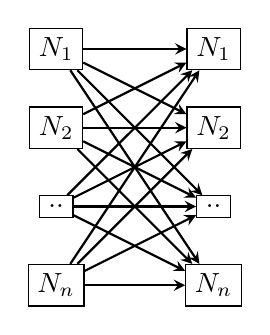
\begin{tikzpicture}[node distance=1cm]
      \node (0A)  [dot]              {$N_1$};
      \node (0B)  [dot, below of=0A] {$N_2$};
      \node (0C)  [dot, below of=0B] {$..$};
      \node (0D)  [dot, below of=0C] {$N_n$};

      \node (1A)  [dot, right of=0A, xshift=1cm] {$N_1$};
      \node (1B)  [dot, right of=0B, xshift=1cm] {$N_2$};
      \node (1C)  [dot, right of=0C, xshift=1cm] {$..$};
      \node (1D)  [dot, right of=0D, xshift=1cm] {$N_n$};

      \draw [arrow] (0A) -- (1A);
      \draw [arrow] (0A) -- (1B);
      \draw [arrow] (0A) -- (1C);
      \draw [arrow] (0A) -- (1D);

      \draw [arrow] (0B) -- (1A);
      \draw [arrow] (0B) -- (1B);
      \draw [arrow] (0B) -- (1C);
      \draw [arrow] (0B) -- (1D);

      \draw [arrow] (0C) -- (1A);
      \draw [arrow] (0C) -- (1B);
      \draw [arrow] (0C) -- (1C);
      \draw [arrow] (0C) -- (1D);

      \draw [arrow] (0D) -- (1A);
      \draw [arrow] (0D) -- (1B);
      \draw [arrow] (0D) -- (1C);
      \draw [arrow] (0D) -- (1D);

    \end{tikzpicture}

    \caption{Naive $n-to-n$ conversion.}
    \label{fig:n-to-n-conversion-boxes-without-intermediate-format}
  \end{subfigure}%
  \begin{subfigure}{.5\textwidth}
    \centering

    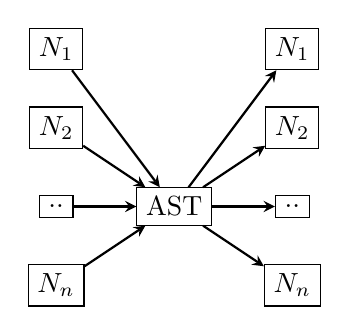
\begin{tikzpicture}[node distance=1cm]
      \node (0A)  [dot]              {$N_1$};
      \node (0B)  [dot, below of=0A] {$N_2$};
      \node (0C)  [dot, below of=0B] {$..$};
      \node (0D)  [dot, below of=0C] {$N_n$};

      \node (mid) [dot, right of=0C, xshift=.5cm] {AST};


      \node (1C)  [dot, right of=mid, xshift=.5cm] {$..$};
      \node (1B)  [dot, above of=1C] {$N_2$};
      \node (1A)  [dot, above of=1B] {$N_1$};
      \node (1D)  [dot, below of=1C] {$N_n$};

      \draw [arrow] (0A) -- (mid);
      \draw [arrow] (0B) -- (mid);
      \draw [arrow] (0C) -- (mid);
      \draw [arrow] (0D) -- (mid);

      \draw [arrow] (mid) -- (1A);
      \draw [arrow] (mid) -- (1B);
      \draw [arrow] (mid) -- (1C);
      \draw [arrow] (mid) -- (1D);

    \end{tikzpicture}

    \caption{$n-to-n$ conversion through intermediate language.}
    \label{fig:n-to-n-conversion-boxes-with-intermediate-format}
  \end{subfigure}
  
  \label{fig:n-to-n-conversion-boxes}
\end{figure}




\section{Conversions are approximations}
\paragraph{A single document have multiple potential interpretations, and can thus be expressed differently within the same output language.} The previous sections may have indicated, that given an input document, there exist a single, unanimous, output document, for each output language. While one could argue the truth of such a statement, this thesis considers it untrue.  The opposition may argue, that if there exist, at least one, semantic difference between two output documents, and these documents are claimed to be expressed in the same language, then these two documents cannot possibly be considered to have derived from the same input document. Subsequently, one would reach the conclusion that these output documents, in fact, are either (a) expressed in two different languages, or (b) derived from two different input documents. This thesis argues the opinion of (b), but claim that the difference stem from differences in the interpretation of the same input document, rather than differences caused by different input documents.

In order to clarify the use of the word ``interpretation'', consider the following example. Assume there exist an abstract idea in the mind of a document author. Assume then that the author encodes this idea using some input language. This thesis employ the philosophical standpoint that the concrete input document (i.e. the encoded idea) is always a compromise (i.e. an approximation) of the actual idea. More precisely put, the input document is always an approximation, attempted to, as precisely as possible, encode the envisioned idea. The intent of the conversion tool is then to translate this approximation of the abstract idea, from the input language, to some output language.  However, since the input document is an approximation of the abstract idea, ambiguity arise, and thus multiple different interpretations of the input document are reasonable. A visualization of the concept is given in Figure \ref{fig:diagram-explaining-interpretations}.

\paragraph{From a more pragmatic perspective, one could argue that allowing multiple interpretations of a single input document, simply, is a necessary prerequisite if one is to achieve the goal of ``writing once, and publishing everywhere''.} The very nature of such a goal implies that the sought documents one wishes to publish (i.e. the ``everywhere''), are different manifestations of some abstract idea (i.e. the ``once''). The statement of the goal, inherently seem to imply, that what is sought is manifestations (i.e. variations) and not mere translations. Consequently, this is the view employed in this thesis.



\begin{figure}[h]
    \centering

    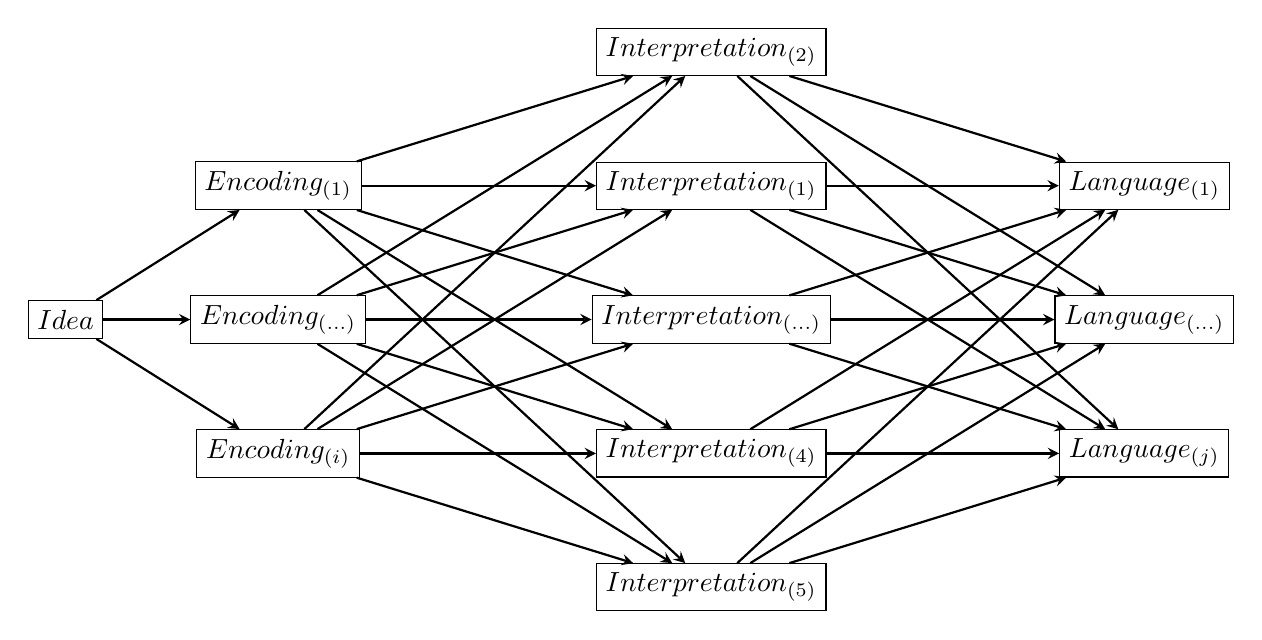
\begin{tikzpicture}[node distance=1.7cm]
      \node (idea)  [dot]            {$Idea$};

      \node (E2)  [dot, right of=idea, xshift=1cm] {$Encoding_{(...)}$};
      \node (E1)  [dot, above of=E2]               {$Encoding_{(1)}$};
      \node (E3)  [dot, below of=E2]               {$Encoding_{(i)}$};

      \node (I3) [dot, right of=E2, xshift=3.8cm] {$Interpretation_{(...)}$};
      \node (I1) [dot, above of=I3]               {$Interpretation_{(1)}$};
      \node (I2) [dot, above of=I1]               {$Interpretation_{(2)}$};
      \node (I4) [dot, below of=I3]               {$Interpretation_{(4)}$};
      \node (I5) [dot, below of=I4]               {$Interpretation_{(5)}$};


      \node (L2)  [dot, right of=I3, xshift=3.8cm] {$Language_{(...)}$};
      \node (L1)  [dot, above of=L2]               {$Language_{(1)}$};
      \node (L3)  [dot, below of=L2]               {$Language_{(j)}$};


      \draw [arrow] (idea) -- (E1);
      \draw [arrow] (idea) -- (E2);
      \draw [arrow] (idea) -- (E3);

      % Encodings to interpretations
      \draw [arrow] (E1) -- (I1);
      \draw [arrow] (E1) -- (I2);
      \draw [arrow] (E1) -- (I3);
      \draw [arrow] (E1) -- (I4);
      \draw [arrow] (E1) -- (I5);

      \draw [arrow] (E2) -- (I1);
      \draw [arrow] (E2) -- (I2);
      \draw [arrow] (E2) -- (I3);
      \draw [arrow] (E2) -- (I4);
      \draw [arrow] (E2) -- (I5);

      \draw [arrow] (E3) -- (I1);
      \draw [arrow] (E3) -- (I2);
      \draw [arrow] (E3) -- (I3);
      \draw [arrow] (E3) -- (I4);
      \draw [arrow] (E3) -- (I5);

      % Interpretations to languages
      \draw [arrow] (I1) -- (L1);
      \draw [arrow] (I1) -- (L2);
      \draw [arrow] (I1) -- (L3);

      \draw [arrow] (I2) -- (L1);
      \draw [arrow] (I2) -- (L2);
      \draw [arrow] (I2) -- (L3);

      \draw [arrow] (I3) -- (L1);
      \draw [arrow] (I3) -- (L2);
      \draw [arrow] (I3) -- (L3);

      \draw [arrow] (I4) -- (L1);
      \draw [arrow] (I4) -- (L2);
      \draw [arrow] (I4) -- (L3);

      \draw [arrow] (I5) -- (L1);
      \draw [arrow] (I5) -- (L2);
      \draw [arrow] (I5) -- (L3);
    \end{tikzpicture}

    \caption{An abstract idea in the mind of the author may be encoded in multiple ways. Any encoding may be interpreted in multiple ways. Any interpretation may be manifested in multiple languages.}
    \label{fig:diagram-explaining-interpretations}
  \end{figure}
% TODO: Perhaps all encodings should not ''arrow to'' all interpretations? Or at least it should be explained?

\paragraph{In order to exemplify the pragmatic usefulness of accepting ambiguous interpretations of input documents, consider an example of a document consisting of a set of paragraphs, intended to be converted to HTML.} One could encode this list of paragraphs, as either a list of \texttt{<li>} elements (i.e. list items), or simply as a set of subsequent \texttt{<p>} elements (i.e. paragraph elements). It is not obvious which one is to be considered the more reasonable, as it depends on how one interprets the subtleties of the input document.

\paragraph{As another example, consider a book, written in some markup language, but intended to be published in HTML.} Perhaps the author wish to publish two versions, where in one, all chapters sequentially follow each other on the same page, and in the other, all chapters are divided into separate pages, hyperlinked to from a table of contents. While both of the output documents are expressed in the language HTML, they are indeed examples variations of the original document. In other words, they exemplify different manifestations of The abstract idea.




\paragraph{Pandoc\footnotePandoc{} handles the ability to produce different output documents from the same input document through two facilities.} One facility is templating, and the other is what the documentation refer to as ``scripting''\footnotePandoc{}. The first essentially refer to the idea of constructing a template into which the input document is fed. Naturally, a unique template as needed for every unique output document. The second facility, scripting, is more general as it operates on a concrete JSON representation of the abstract syntax tree, i.e. what has previously been referred to as the intermediate language.

A visual interpretation of these facilities of Pandoc\footnotePandoc{} is depicted in Figure \ref{fig:interpretation-of-pandoc}.

The main problem of the scripting approach of Pandoc\footnotePandoc{}, is that it is, as outlined by \citet{krijnen}, coupled to this intermediate language. As \citet{krijnen} suggest, it is ``unrealistic to expect that it can represent all document elements which are introduced by any of the existing or future standards''.

\citet{krijnen} suggest a less naive approach, that demonstrate how conversion schemes can be shared across different input and output languages, through working with grammars and a set of Haskell libraries. The main benefit of such an approach is that it enables flexible package sharing, in ways is similar to the eco-system of \LaTeX{} \citep{krijnen}.



\begin{figure}[h]
    \centering

    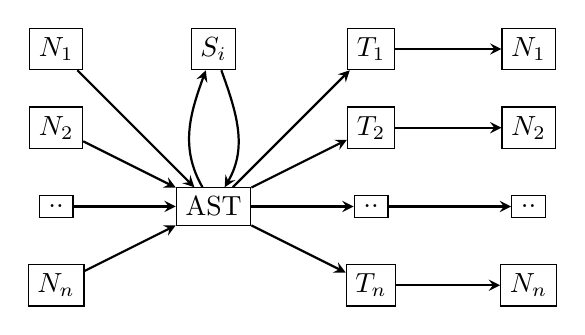
\begin{tikzpicture}[node distance=1cm]
      \node (0A)  [dot]              {$N_1$};
      \node (0B)  [dot, below of=0A] {$N_2$};
      \node (0C)  [dot, below of=0B] {$..$};
      \node (0D)  [dot, below of=0C] {$N_n$};

      \node (mid) [dot, right of=0C,  xshift=1cm] {AST};
      \node (ext) [dot, above of=mid, yshift=1cm] {$S_i$};

      \node (1C)  [dot, right of=mid, xshift=1cm] {$..$};
      \node (1B)  [dot, above of=1C] {$T_2$};
      \node (1A)  [dot, above of=1B] {$T_1$};
      \node (1D)  [dot, below of=1C] {$T_n$};

      \node (2C)  [dot, right of=1C, xshift=1cm] {$..$};
      \node (2B)  [dot, above of=2C] {$N_2$};
      \node (2A)  [dot, above of=2B] {$N_1$};
      \node (2D)  [dot, below of=2C] {$N_n$};

      \draw [arrow] (0A) -- (mid);
      \draw [arrow] (0B) -- (mid);
      \draw [arrow] (0C) -- (mid);
      \draw [arrow] (0D) -- (mid);

      \draw [arrow] (mid) to[out=120, in=-110] (ext);
      \draw [arrow] (ext) to[out=-70, in=60] (mid);

      \draw [arrow] (mid) -- (1A);
      \draw [arrow] (mid) -- (1B);
      \draw [arrow] (mid) -- (1C);
      \draw [arrow] (mid) -- (1D);

      \draw [arrow] (1A) -- (2A);
      \draw [arrow] (1B) -- (2B);
      \draw [arrow] (1C) -- (2C);
      \draw [arrow] (1D) -- (2D);

    \end{tikzpicture}

    \caption{Interpretation of the Pandoc workflow when making use of the templating ($T_n$) and scripting ($S$) facilities.}
    \label{fig:interpretation-of-pandoc}
  \end{figure}



\paragraph{To summarize, this thesis will concern itself with four types of conversions -- conversions from input language (i.e. encoding) to interpretation, conversions from interpretations to interpretations, translations from interpretations to interpretations (not yet discussed), and conversions from interpretations to output languages.} In other words, this thesis will concern itself only very briefly with conversions from the abstract idea to encodings (i.e. input languages). 







\section{Markup has resolution}

\paragraph{This thesis is based upon the hypothesis that there exist a hierarchy of abstraction, in which conversions are trivial in one direction but significantly more complex in the other.} Call the complex direction ``up'', and the trivial ``down''. If true, then it must be considered futile to attempt to convert ``up'' in the chain, and if converting ``up'' is futile, then it must be considered a priority to express all documents, in potential need of conversion, in a language as ``high'' up in the abstraction chain as possible. 

\paragraph{It has already been argued that markup languages can be categorized according to properties, and it is such properties must determine whether a given language is more abstract than another, i.e. weather one language can be converted to another or not.}
An example of such a categorization is whether a language is presentation-oriented or not. One could argue, that the idea of presentation is a specialization, where the idea of describing a thing outside of its domain of presentation is an abstraction. This would mean, that languages concerned with presentation are less abstract (i.e. more specialized) than those not concerned with presentation.

The classical notion of ``separation of concerns'' emphasizes the known benefits of such a strategy. Thus, the separation of presentation and content not only makes intuitive sense, but have also been successfully applied in the real-world. Consider for example how CSS has successfully separated presentation from content in HTML\footnote{http://www.w3.org/standards/webdesign/htmlcss\#whatcss}.

Converting from a non-presentational language to a presentational language is a conversion ``down'' the abstraction chain, if ``level of presentational coupling'' is used as the categorizing property when differentiating between two different languages. Vice versa, the task of converting from a presentational language to a non-presentational language is a conversion ``up'' the abstraction chain. Thus, the latter must be considered a significantly more difficult task than the former, assuming the hypothesis of this thesis is true.

\paragraph{The hypothesis is not merely that presentation and content are different,} but again, that all languages exhibit properties, and that all of these properties can be grouped into categories, where these categories can be ordered hierarchically according to their level of abstraction.

\paragraph{The chain of abstractions is perhaps better explained by analogy of a tree,} rather than a chain. Consider Figure \ref{fig:fictive-specialization-tree}, in which the language $L$ is the most abstract, and the languages ``below'' are specializations of that language. It is important to understand that, like in any hierarchy, branchings may exist. Which becomes apparent through considering the siblings $L1$, $L2$ and their relationship. However, it is also important to remember that the hypothesis suggest to only allow conversions from parent to child (i.e. ``down'') and never from child to parent (i.e. ``up''), nor from child to child (i.e. ``sideways'').

\begin{figure}[h]
  \centering
  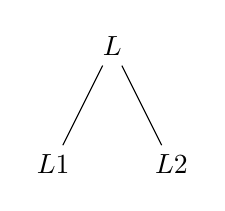
\begin{tikzpicture}[
    tlabel/.style={pos=1,right=2pt,font=\footnotesize\color{red!70!black}},
      sibling distance=1.5cm,
    ]
    \node {$L$}
    child {node {$L1$}}
    child {node {$L2$}}
    ;
  \end{tikzpicture}

  \caption{Fictive tree of abstraction, over the three languages $\{L, L1, L2\}$.}
  \label{fig:fictive-specialization-tree}
\end{figure}

\paragraph{Consider the following concrete example of the three languages HTML, \LaTeX{}, and Markdown.} Figure \ref{fig:hierarchy-of-abstraction-example-tree} depicts one potential interpretation of the relationship between the three languages. The word \emph{one} is used instead of \emph{the} to emphasize that this particular relationship might not hold when considering all properties of these languages. The figure is to be considered an oversimplified example.

HTML is (in Figure \ref{fig:hierarchy-of-abstraction-example-tree}) depicted as the parent language (i.e. the most abstract), while \LaTeX and Markdown, are depicted as children (i.e. derivations) of that language (and are thus more specialized). The hypothesis thus suggests that converting from HTML to either \LaTeX{} or Markdown should be considered a ``safe'' task, while all other conversions (i.e. ``up'' or ``sideways'') should be considered ``unsafe''.

Consider then the concrete sentence (or rather: document fragment) expressed in all of these languages (still Figure \ref{fig:hierarchy-of-abstraction-example-tree}). The fragment, expressed in HTML, employ the use of the two distinct elements \texttt{em} (emphasis) and \texttt{i} (italics). While these two, in web browsers, render the same, the following quote, from the HTML5 specification,\footnote{http://www.w3.org/TR/html5/text-level-semantics.html\#the-em-element} explain the existence of a semantic difference.

\begin{quote}
``The \emph{em} element isn't a generic \emph{italics} element. Sometimes, text is intended to stand out from the rest of the paragraph, as if it was in a different mood or voice. For this, the \emph{i} element is more appropriate.''
\begin{flushright}
% TODO Make sure all quotes are languageted alike
\textit{-- HTML5 Recommended specification 2014}
%TODO: Ref
\end{flushright}
\end{quote}

The semantic encapsulation of the word ``Cats'' (in the document fragment depicted in Figure \ref{fig:hierarchy-of-abstraction-example-tree}) is thus intended to be different from the semantic encapsulation of the word ``Dogs'' (as they are surrounded by tags with different semantic meaning). The existence of such a difference is the key to understanding the relationship between the abstraction of two languages.

\begin{figure}[h]
  \centering
  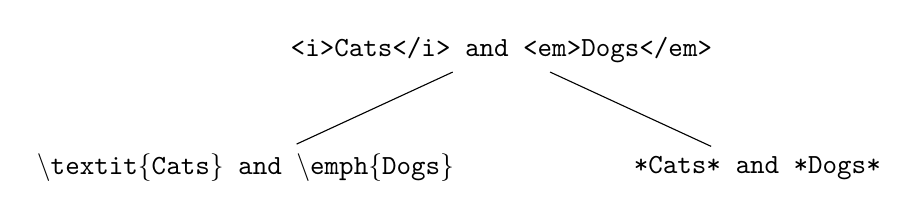
\begin{tikzpicture}[
    tlabel/.style={pos=1,right=2pt,font=\footnotesize\color{red!70!black}},
      sibling distance=6.5cm,
    ]
    \node {
      \texttt{<i>Cats</i> and <em>Dogs</em>}
    }
    child {node {
      \texttt{\textbackslash textit\{Cats\} and \textbackslash emph\{Dogs\}}
    }}
    child {node {
      \texttt{*Cats* and *Dogs*}
    }}
    ;
  \end{tikzpicture}

  \caption{Hierarchy of abstraction of the three languages HTML, \LaTeX, and Markdown (top-to-bottom, left-to-right).}
  \label{fig:hierarchy-of-abstraction-example-tree}
\end{figure}

\paragraph{Preservation of the ability to distinguish all elements of different semantic types, should determine whether a string in a language can or cannot be converted to another language.}

Converting the fragment (of Figure \ref{fig:hierarchy-of-abstraction-example-tree}) expressed in HTML to \LaTeX{} poses no immediate problem, since the distinction can be preserved. Converting the fragment expressed in HTML to Markdown, however, pose problems since the distinction cannot possibly be preserved, due to the less rich expressiveness of Markdown. Thus, HTML must (in this simplified example) be considered the more abstract language, and Markdown the more concrete (i.e. less abstract).

To generalize: If a distinction cannot be preserved when converting from language $A$ to language $B$, then $A$ must be considered the relatively superior (i.e. the more abstract) language.

\paragraph{Preserving difference is more fundamental than equivalence.} While the semantic meaning of the markup keywords (actually macros) \texttt{textit} and \texttt{emph} in the language \LaTeX{} might not refer to the exact same semantic meaning as \texttt{i} and \texttt{emph} of HTML, the importance lies in the preservation of the distinction. If one were to only convert between languages that preserved the exact same semantic meaning, constructing an abstraction tree would be a much more difficult task. Simply because semantic equivalence is a philosophically more difficult question, than syntactic difference. Thus, this thesis explore the concept of preservation of semantic difference (through preservation of syntactic difference), and leave semantic equivalence open for future research.
\label{sec:difference-is-more-important-than-equivalence}

%TODO: The conversion is the semantically closest, and distinction is preserved.

\paragraph{Conversions ``up'' and ``sideways'' are impossible because distinction may have been lost.} Expanding on the idea that a conversion that cause loss in semantic distinction must be considered a conversion ``down'' the abstraction chain, it becomes apparent that conversions in the opposite direction mean converting from a language with ``less information'' to one with more. Analogy to \emph{resolution} may spawn good understanding. An image of 200x200 pixels may very well be scaled down to 20x20 pixels. However a 20x20 pixels cannot possibly be intelligently scaled up to 200x200 pixels. Simply because the 20x20 pixel image contain ``less information'' than needed to express the original image in 200x200 pixels.

The number of semantically different syntactical constructs of a language, perfectly map to the analogy of number of pixels carrying information. As pixels carrying information are destroyed, there is no way to recreate them.

There are of course instances where converting from a low-resolution language to a high-resolution pose no problem at all. Consider for example a 200x200 pixels perfectly black image. Scaling this image down to a resolution of 20x20 pixels, and then scaling it back up to a resolution of 200x200 pose no problem at all. The final image is exactly the same as the original. Consider then on the other hand a 200x200 pixel portrait photograph. Scaling this image down to a resolution of 20x20, and then scaling it back up to 200x200 cause serious information loss. The final image is now merely an approximation of the original.


\paragraph{Thus, retainment of distinction between two languages must be determined on the basis of all syntactical constructs of a language, and not merely those utilized in particular instances.}
In the language of pixels, it is trivial to imagine cases where conversions from low resolution to high resolution indeed cause no loss of information (consider the black square). However, this is, again, a fortunate effect of the specific case. It is equally trivial to imagine a counter-example, where in the same language, such a conversion will cause loss of information (consider the portrait photograph).

The same apply to markup languages. It is trivial to imagine an example where conversion from a low-resolution language (e.g. Markdown) to a high-resolution language (e.g. HTML) will cause no information loss. Consider for example how all information is retained in Figure \ref{fig:low-to-high-resolution-non-destructive}. However, as with pixel resolution, it is equally trivial to imagine an example where information (i.e. distinction) is in fact lost. Consider for example how information is lost in Figure \ref{fig:low-to-high-resolution-destructive}.


\begin{figure}[h]

\begin{subfigure}{.5\textwidth}
  \centering
  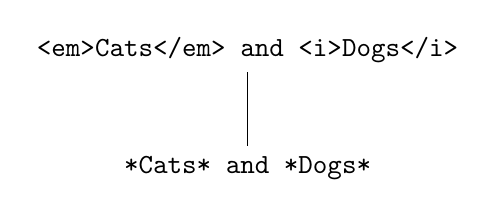
\begin{tikzpicture}[
    tlabel/.style={pos=1,right=2pt,font=\footnotesize\color{red!70!black}},
      sibling distance=6.5cm,
    ]
    \node {
      \texttt{<em>Cats</em> and <i>Dogs</i>}
    }
    child {node {
      \texttt{*Cats* and *Dogs*}
    }}
    ;
  \end{tikzpicture}

  \caption{Example of an instance where converting ``up'' the abstraction chain do cause loss of information.}
  \label{fig:low-to-high-resolution-destructive}
\end{subfigure}%
\begin{subfigure}{.5\textwidth}
  \centering
  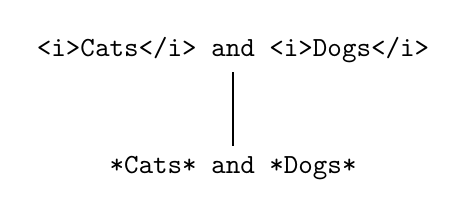
\begin{tikzpicture}[
    tlabel/.style={pos=1,right=2pt,font=\footnotesize\color{red!70!black}},
      sibling distance=6.5cm,
    ]
    \node {
      \texttt{<i>Cats</i> and <i>Dogs</i>}
    }
    child {node {
      \texttt{*Cats* and *Dogs*}
    }}
    ;
  \end{tikzpicture}

  \caption{Example of an instance where converting ``up'' the abstraction chain does not cause loss of information.}
  \label{fig:low-to-high-resolution-non-destructive}
\end{subfigure}

\caption{Example of how conversions from low resolution to high resolution can not be guaranteed to not cause loss of information.}
\end{figure}


\paragraph{Conversions where the number of semantic distinctions before and after the conversion remain exactly the same,} is what this thesis refer to as a translation. 



%\color{red}
%\section{Destructive and non-destructive conversions}
%TODO. Scaling down vs. simply converting the image within the same resolution.

%\section{Conversions inside or outside the bounds of a language}
%\label{sec:conversions-in-or-out-of-languages}
%TODO. 
%\color{black}




\section{Generality of markup conversion programs}
\label{sec:theory-of-document-processing}
\label{sec:microframework}
\paragraph{Markup conversion programs can be categorized according to their level of generalization.} Oversimplified, a markup conversion program can be seen as a function that takes some document, expressed in some language, as input, and produce some document, expressed in some language, as output, where these languages may very well be different or the same. In terms of Equation \ref{eq:microframework-i-o}, $P$ maps documents from the domain $\mathbb{I}$ to documents in the domain $\mathbb{O}$, where there may be an overlap between $\mathbb{I}$ and $\mathbb{O}$.

\begin{equation}
  P : \mathbb{I} \rightarrow \mathbb{O}
  \label{eq:microframework-i-o}
\end{equation}

In order to discuss the body of all possible markup conversion programs, consider Equation \ref{eq:microframework-n-n} rather than \ref{eq:microframework-i-o}. If $\mathbb{N}$ is the domain of all possible markup languages, then the conversion program $P$ can take the form of any conceivable conversion program that maps some input markup language to some output markup language.

\begin{equation}
  P : \mathbb{N} \rightarrow \mathbb{N}
  \label{eq:microframework-n-n}
\end{equation}

In order to reason about the generality of conversion programs, assume that all markup conversion programs over the domain $\mathbb{N}$ can be considered to take generalized or specialized input, and then produce generalized or specialized output. Generalized input, would mean that the program in question can take any markup language of the domain $\mathbb{N}$ as input, whereas specialized would mean that it only can take some subset. The same reason applies to the output language. Exhausting all the permutations of these, yield four different types of conversion programs, as depicted through a quadrant diagram in Figure \ref{fig:microframework-quadrant}.


\begin{figure}[h]
  \centering

  \def\arraystretch{1.5}
  \begin{tabular}{r|c|c}

    & \textbf{Generalized out} & \textbf{Specialized out} \\ \hline

    \textbf{Generalized in} &
     A
    &
     C

    \\ \hline

    \textbf{Specialized in} &
     B
    &
     D

    \\ 
  \end{tabular}

  \caption{Exhausting the permutations of generalization levels, on a binary scale where input and output is considered either generalized or not.}
  \label{fig:microframework-quadrant}
\end{figure}




\paragraph{Quadrant D programs take specialized input, and produce specialized output,}
and are thus really specialized conversion programs. Conversions are always made from a specific subset, to a specific subset. If these subsets are the same, then the program is one that can create variants of a document within the same language.

The problem however, is of course that if an author wishes to utilize some input or output language outside of the subset, a completely new program is required.

Examples of such a program may for example be a \LaTeX{}-to-PDF converter, or a Markdown-to-HTML converter, and is generally visualized in Figure \ref{fig:workflows-framework-spec-in-spec-out}.


\paragraph{Quadrant C programs take generalized input, and produce specialized output,} and thus contain a, quite odd, set of conversion programs, that, take input from any subset, but always output languages of a specific subset. If one would need to output a language from a different domain, then the program need to be rewritten.

Such a program might for example be an ``anything-to-XML converter'', that simply encapsulates any string with a root tag and escapes any XML-like syntax from the input string in order to avoid syntax errors. Consequently the program would be able to receive any language, and yet always be able to output valid XML. Such a program is generally visualized in Figure \ref{fig:workflows-framework-gen-in-spec-out}.





\begin{figure}[h]
\begin{subfigure}{.25\textwidth}

  \centering

  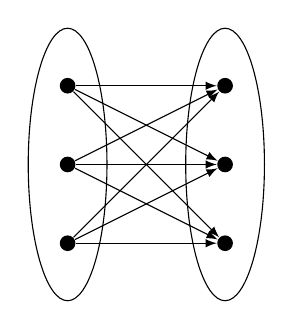
\begin{tikzpicture}
  %put some nodes on the left
  \foreach \x in {1,2,3}{
    \node[fill,circle,inner sep=2pt] (l\x) at (0,\x) {};
  }
  \node[fit=(l1) (l2) (l3),ellipse,draw,minimum width=1cm] {}; 

  %put some nodes on the right
  \foreach \x[count=\xi] in {1,2,3}{
    \node[fill,circle,inner sep=2pt] (r\xi) at (2,\x) {};
  }
  \node[fit=(r1) (r2) (r3),ellipse,draw,minimum width=1cm] {};

  \draw[-latex] (l3) -- (r3);
  \draw[-latex] (l3) -- (r2);
  \draw[-latex] (l3) -- (r1);
  \draw[-latex] (l2) -- (r3);
  \draw[-latex] (l2) -- (r2);
  \draw[-latex] (l2) -- (r1);
  \draw[-latex] (l1) -- (r3);
  \draw[-latex] (l1) -- (r2);
  \draw[-latex] (l1) -- (r1);
  \end{tikzpicture}

  \caption{n-n}
  \label{fig:workflows-framework-gen-in-gen-out}

\end{subfigure}%
\begin{subfigure}{.25\textwidth}

  \centering

  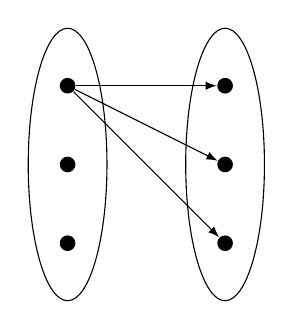
\begin{tikzpicture}
  %put some nodes on the left
  \foreach \x in {1,2,3}{
    \node[fill,circle,inner sep=2pt] (l\x) at (0,\x) {};
  }
  \node[fit=(l1) (l2) (l3),ellipse,draw,minimum width=1cm] {}; 

  %put some nodes on the right
  \foreach \x[count=\xi] in {1,2,3}{
    \node[fill,circle,inner sep=2pt] (r\xi) at (2,\x) {};
  }
  \node[fit=(r1) (r2) (r3),ellipse,draw,minimum width=1cm] {};

  \draw[-latex] (l3) -- (r1);
  \draw[-latex] (l3) -- (r2);
  \draw[-latex] (l3) -- (r3);
  \end{tikzpicture}

  \caption{1-n}
  \label{fig:workflows-framework-spec-in-gen-out}

\end{subfigure}%
\begin{subfigure}{.25\textwidth}

  \centering

  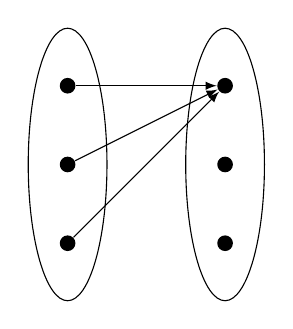
\begin{tikzpicture}
  %put some nodes on the left
  \foreach \x in {1,2,3}{
    \node[fill,circle,inner sep=2pt] (l\x) at (0,\x) {};
  }
  \node[fit=(l1) (l2) (l3),ellipse,draw,minimum width=1cm] {}; 

  %put some nodes on the right
  \foreach \x[count=\xi] in {1,2,3}{
    \node[fill,circle,inner sep=2pt] (r\xi) at (2,\x) {};
  }
  \node[fit=(r1) (r2) (r3),ellipse,draw,minimum width=1cm] {};

  \draw[-latex] (l3) -- (r3);
  \draw[-latex] (l2) -- (r3);
  \draw[-latex] (l1) -- (r3);
  \end{tikzpicture}

  \caption{n-1}
  \label{fig:workflows-framework-gen-in-spec-out}

\end{subfigure}%
\begin{subfigure}{.25\textwidth}

  \centering

  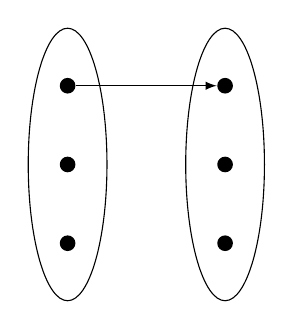
\begin{tikzpicture}
  %put some nodes on the left
  \foreach \x in {1,2,3}{
    \node[fill,circle,inner sep=2pt] (l\x) at (0,\x) {};
  }
  \node[fit=(l1) (l2) (l3),ellipse,draw,minimum width=1cm] {}; 

  %put some nodes on the right
  \foreach \x[count=\xi] in {1,2,3}{
    \node[fill,circle,inner sep=2pt] (r\xi) at (2,\x) {};
  }
  \node[fit=(r1) (r2) (r3),ellipse,draw,minimum width=1cm] {};

  \draw[-latex] (l3) -- (r3);
  \end{tikzpicture}

  \caption{1-1}
  \label{fig:workflows-framework-spec-in-spec-out}

\end{subfigure}%

  \caption{Function mappings for hypothetical instances of markup conversion programs, exemplifying different levels of generality.}
  \label{fig:conversion-generality-function-mapping}
\end{figure}





\paragraph{Quadrant B programs take specialized input, and produce generalized output,}
and thus resemble the widely employed combination of XML and XSLT. Authors can express a document in some arbitrary XML language and then employ XSLT as a means of converting the document into multiple different output languages. Such a program is generally visualized in Figure \ref{fig:workflows-framework-spec-in-gen-out}.


\paragraph{Quadrant A programs take generalized input, and produce generalized output,}
and thus represent the most general kind of markup conversion programs. They take input in any language of the domain $\mathbb{N}$ and can produce output in any of the languages of the domain $\mathbb{N}$. An example program that exhibits this behavior is the widely used software Pandoc\footnotePandoc{}. Naturally, Pandoc\footnotePandoc{} is, of course, a pragmatic compromise and does not convert from every conceivable language to every conceivable language. However, it is perhaps the most successful effort in the area yet, and thus also serve as an example of the non-triviality associated with $n-to-n$ conversion. Such a program is generally visualized in Figure \ref{fig:workflows-framework-gen-in-gen-out}.



\paragraph{In a perfect world, conversion programs would painlessly convert any language to any language and thus exist in  Quadrant A.} However, as implied in the beginning of this thesis -- writing a pragmatically useful Quadrant A program is not trivial because converting any language to any language will require conversions from languages with lower semantic resolution to those with higher, which this thesis argue is an impossibility.

Consequently, this thesis instead explores quadrant B programs, and attempts to identify the properties required for a program, and its corresponding input language, to enable $1-to-n$ conversions while, to the greatest extent possible, only converting ``down'' the abstraction chain (i.e. from higher resolution, to lower resolution).


% TODO: Should I actually write about this?
% \section{Situational analysis}
% In this section we will criticize some of the common workflows through employing the quadrant approach already introduced and depicted by Figure \ref{fig:microframework-quadrant}. \emph{(TODO) I will probably remove this section, because I assume the reader has already appreciated the costs of working outside of the A quadrant.}
% Why are so many documents still procedural?
% Model information flows of contemporary publishing. Figures describing the current state in contrast to the thesis's subjective idea of the ideal state. Refer to Reid (1980).

% \subsection{Presentational}
% i.e. Microsoft Word etc.
% [FIG. ]
% Explicit outline of the problems so that we can attack them in the hypothetical ideal.

% \subsection{Procedural}
% i.e. \LaTeX etc.
% [FIG. ]
% Explicit outline of the problems so that we can attack them in the hypothetical ideal.

% \subsection{Descriptive}
% i.e. DocBook, EPUB, Markdown etc.
% [FIG. ]
% Explicit outline of the problems so that we can attack them in the hypothetical ideal.

% \subsection{A hypothetical ideal addressing the problems}
% [FIG.]

% \subsubsection{Composition \& Abstraction}
% The minimal denominator.









% \section{Language conversion as a series of pipes}
% \color{red}
% \paragraph{Instead, consider the following idea.} Let $N$ be all the languages an author may want to convert to. Let all the concrete languages of $N$ be represented by $n_1, n_2, .., n_n$. Let $M$ be some subset of the languages in $N$ (i.e. $M \subseteq N$). Such that the languages of $M$ exhibit only language properties also exhibited by all languages of $N$. In other words, any string in $M$ must be expressible in any of the languages $n_1, n_2, .., n_n$. In other words, $M$ is a subset of the intersection of all languages in $N$, i.e: $M \subseteq (n_1 \cap n_2 \cap .. \cap n_n)$.

% TODO:
% However, we are only informally talking about sets and subsets here. Since most languages that we want to convert to (e.g. XML, LaTeX) are definitely not regular they are thus at least context-free. In the Chomsky Hierarchy. And since context-free grammars are not closed under language inclusion, this mean we cannot actually certainly say that some language actually is a subset of another language.

%\paragraph{This thesis suggest an approach that can be similar to a pipeline of template}, much like the notion of UNIX pipes\footnote{http://en.wikipedia.org/wiki/Pipeline\_(Unix)}), and through this achieve a high level of composability. Instead of a one-pass-conversion, conversions are split into composable chunks at different levels of abstraction. But all this will be discussed further on in the thesis.

%\color{black}
% TODO: Returning to black, to mark end of potentially deprecated section.
























\chapter{Problem and hypothesis}
To summarize, the problem focus of this thesis is three-fold.

\begin{itemize}
\item Many languages exist, and converting documents between these languages is non-trivial.
\item Sharing packages/modules (i.e. code) for commonly performed conversions (across) language-boundaries is non-trivial.
\item Allowing multiple interpretations, and thus output documents, to stem from the same input document, is non-trivial.
\end{itemize}




\paragraph{The argument is that conversion tools that intelligently respects the resolution of markup languages mitigate these problems.} Thus, it is the aim of this thesis to show that it is possible to construct an eco-system of conversion tools that facilitate the respecting of resolution, through identifying a highly abstract language, and enable the dissecting of conversions into utterly small increments. As the proof will be deduced from example, the aim is only to demonstrate the possibility of such an approach. Suitability of the particular, suggested, approach will not be verified.

\paragraph{The hypothesis is, thus, that it is possible to construct an eco-system of tools, that through respecting semantic resolution, allow authors to:}

\begin{enumerate}
\item write once and publish everywhere (i.e. convert to any language), and
\item share common conversions as packages across output language boundaries (e.g. generation of tables of contents), while
\item allowing ambiguous interpretations, such that the same input document may have several output documents in a given language.
\end{enumerate}



\section{Deliverables}
In order to meet the research goal of proving the possibility of converting markup while respecting resolution, the following concrete results has been delivered.

\paragraph{Deliverable I.} This thesis identifies a potential workflow, that enable the respecting of markup resolution, allow for sharing of conversion packages, while still being able to produce any output language.

\paragraph{Deliverable II.} This thesis identifies some fundamental characteristics, required, for a markup language, to have a relatively high enough semantic resolution, as to be used as an input language when converting to common output languages today.

\paragraph{The first deliverable is exemplified through a workflow model, and a step-by-step usage example, showcasing relevant pieces of program code. Whereas the second deliverable is mainly provided as a set of requirements, but is also complemented with some relevant pieces of program code that exemplify a potential implementation.}





\section{Method}
The research goals have been met through analyzing foundational characteristics of common, current, and previous, markup languages, as well as strengths and fallacies of existing conversion techniques. Publications on historically significant markup languages have been analyzed, whereas standards specifications, documentation, and more informal publications have been analyzed for more recent languages. All research in this thesis is to be considered qualitative.


\section{Delimitations}
\begin{itemize}
\item Document validation (e.g. Document Type Definitions) is not be explored in detail.
\item Neither white-space, nor character encoding is explored in detail.
\item Some implementation details are consciously ignored, as only a prototype is developed.
\end{itemize}







%\section{Thesis outline}
%\color{red}
%This thesis is centered around two major contributions. A new markup language, and a model for markup conversion.

%The high-level goals already introduced in this background chapter is aimed to guide these two contributions, and will constantly be returned to, and reflected upon, throughout the thesis.

%The chapters following the initial Background chapter will come in pairs, where the first is aimed toward the first contribution and the second toward the second.

%The first set of pairs is a look into different important theoretical concepts of the two. Thus characteristics of markup languages, and characteristics of document processing.

%The second set of pairs derive requirements from this first pair, in other words from the existing body of theory. These requirements are posed on the two major contributions.

%The third and last set of pairs engineer the two contributions using both the requirements and previously discussed theory as a basis for argument.

%Finally the thesis is finished off with the usual conclusions, analysis, and discussions.
%\color{black}

























% % % % % % % % % % % % % % % % % % % % % % 
%
%
%
%   Theory: Characteristics of markup languages
%   and language conversion
%
%
%
% % % % % % % % % % % % % % % % % % % % % %


\chapter{Theory -- characteristics of markup languages and language conversion}
\label{sec:theory}
This chapter explores and explains some of the most important characteristics of markup languages.








\section{A Taxonomy of Markup Languages}
\label{sec:taxonomy}
\paragraph{In \citeyear{coombs}, \citeauthor*{coombs} published an article dubbed \textit{Markup Systems and the Future of Scholarly Text Processing}. While the intent of the article, presumably, was to speculate on the future of markup -- it also provided a solid taxonomy of markup languages.} This thesis utilize the categorizations of ``types of markup'' identified by \citet{coombs}, under the term ``markup theory''. \citet{coombs} divide markup languages into the three categories (1) Punctuational, (2) Presentational, (3) Procedural, (4) Descriptive, and (5) Abstract. The following sections will further explore these categories.

Intermingled in these explanations are also opinions from \citet{bray} -- co-founder of the Open Text Corporation, and co-author of the first XML 1.0 draft specification. The opinions of \citeauthor{bray} was expressed in a blog post exploring the categorizations of \citet{coombs}. It is \citeauthor{bray} that described the work of \citeauthor{coombs} as a ``taxonomy''. The opinions of \citeauthor{bray} are intermingled, both because they contemporize the work of \citeauthor{coombs}, but also because there are some conflicts of opinion between the two, which shed light on how the lines between each category in the taxonomy is yet too vaguely defined, and thus cause fragmentation. While the statements of \citeauthor{bray} are informal in nature, his history in the field bestow him reliability and serve the purpose of emphasizing fragmentation well. 


\subsection{Punctuational}
\paragraph{Punctuational markup refer to the markup that is paid very little attention to in everyday life. Spaces, commas, periods, words, sentences, and so forth.} As \citet{coombs} points out, punctuational markup has been studied by mankind for hundreds of years. The example \citet{coombs} use to underline that punctuational markup should, indeed, be considered markup and not merely a part of our writing system -- is the following. Consider the all the conflicting opinions on how punctuational markup should be used. One argue it ought to be a  semicolon, another argue it should be a colon. One argue space-delimited dash, another argue dash with no space. Consider the author contemplating whether a certain domain of sentences/words should be presented as \textbf{bold} or as \textit{italics}. This is the same kind of choice, as the mentioned choices between semicolon, colon and so forth. However, today, \textbf{bold} and \textit{italics} can clearly be considered markup in languages such as HTML. But the 

Understand, that the term punctuational markup, according to \citet{coombs}, does not refer to the idea of encoding punctuation in some other language (i.e. ``\texttt{\&mdash;}'') but rather the actual punctuation itself (i.e. ``\texttt{--}''). In other words, the use of for example character entities in HTML5\footnote{http://dev.w3.org/html5/html-author/charref} is not to be considered punctuational markup. Rather, if using the the actual dash character and its surrounding space characters is the punctuational markup.




\subsection{Presentational}
\paragraph{Consider a document written on a very old, mechanical typewriter. Presentational markup, according to \citet{coombs} refer to the practice where the author of a document (e.g.) hit the space key multiple times to center text on the page.} Another example would be to hit the carriage return key multiple times in order to delimit paragraphs or extend line-breaks.

Now, consider a physical paper document written with a ball pen by hand. With a little bit of effort the author can easily distinguish two parts of the text by applying the technique of writing in italics, or even in cursive. So the reader of the document would understand that author is attempting to communicate some semantic difference between the non-italic and the italic parts.

To understand presentational markup, consider the two above cases -- the typewriter document and the handwritten document. In both cases the presentational elements is embedded within the language of the document. The semantics intended by the author (e.g. a paragraph break) is achieved through presentational means.

\citet{bray} makes the concept of presentational markup, more clear by referring to older What You See Is What You Get (WYSIWYG) word processors. Since modern word processors work with (e.g.) descriptive markup ``under the hood'', this analogy generally no longer holds. But for the sake of the argument, imagine some really old version of a visual word processor. By surrounding parts of a document with code specific to a particular word processor that particular word processor would know to (e.g.) display that piece of text centered, in bold, in italics or so forth.

One immediate problem with this, the quick reader probably have noticed, can be extracted from one particular sentence -- ``a specific word processor''. Presentational markup requires standardization of what codes to use to mark things such as bold, breaks, sizes and so forth. As you can probably imagine, with the creativity of programmers, and proprietary incentives, this quickly gets out of scale.

\subsubsection{Implicitness}
Another more subtle issue, not mentioned by neither \citet{coombs} nor \citet{bray}, is that of implicitness. As the presentational codes of WYSIWYG word processors are not actually visible to the user of the interface -- there exist a mental disconnect. Consider for example the concept of a paragraph break, and the concept of a hard line-break. Now, assume that, in a particular editor, a paragraph break has the same visual appearance as two consecutive hard line-breaks. If one author types up a document, and hands it to another author. How could the second author possibly know whether the first author have employed paragraph breaks or hard line-breaks? Perhaps it is this problem that \citet{bray} refer to, when arguing that What You See Is What You Get essentially is a false claim.
%TODO: This claim seems to be false! I have misunderstood and this need to be rethought.



\subsection{Procedural}
\paragraph{The notion of Procedural markup is perhaps most easily explained through analogy to procedural programming.} Essentially, procedural markup refers to the idea of embedding code instructions directly in a document.

Much as in procedural languages, code duplication, or painful repetition, \citet{bray} argue, can be reduced through elaborate macros or subroutines.

This is the first category, of this chapter, that actually show the user an abstraction of a particular concept rather than the actual concept. Assume an author is to write a particular sentence in a red font. If done through presentational markup, the user would actually see the sentence in red. If however done through procedural markup the user would see some code instruction that indicated the switching to the color red, perhaps as depicted in Figure \ref{fig:procedural-markup-red-sentence}.


\begin{figure}[h]
\centering
\fbox{
\texttt{
  \textbackslash color\{red\} This is a red sentence.
  }
}
\caption{An example of procedural markup in the language \LaTeX{}.}
\label{fig:procedural-markup-red-sentence}
\end{figure}


\begin{figure}[h]
\centering
\fbox{
\texttt{
  .sk 3 a;.in +10 -10;.ls 0;.cp 2 Multiple instructions.
  }
}
\caption{An example of procedural markup, as given by \citet{coombs}.}
\label{fig:procedural-markup-coombs}
\end{figure}



Depending on the syntax of the language, procedural markup might also turn out like a mess of symbols where a human may have a hard time cognitively separating the compiler instructions from the actual plain-text. \citet{coombs} gives an example of procedural markup, as can be seen in Figure \ref{fig:procedural-markup-coombs}, and suggest that the instructions should be interpreted as follows:

\begin{enumerate}
\item Skip three lines -- the equivalent of double-spacing twice.
\item Indent ten columns from the left and ten columns from the right.
\item Change to single-spacing.
\item Start a new page if fewer than two lines remain on the current page.
\end{enumerate}

While the syntax of course is parseable for a computer, it is all but trivial for the untrained human to read. Without syntax highlighting it is even quite hard to give the string of of Figure \ref{fig:procedural-markup-red-sentence} text a glance and quickly figure out what parts are instructions and what parts are characters.

\subsubsection{Mutation}
An interesting problem that reasonably may cause mental overhead for a document author working with procedural markup, is that of side-effects. Arguably, the notion of ``mutation'' or ``side-effects'' is a great source of power in programming, but also a great source of frustration. Programs that frequently mutate are often tricky to debug.

The same is true for procedural markup. The code instruction in Figure \ref{fig:procedural-markup-red-sentence} could be informally described as ``switch to the red pen, from now and onwards''. If the author of a document only intended to mark some substring as red and not the entire rest of the document in red, then the author must remember to switch back to whichever color the document was in before the instruction.

To exemplify the problem -- assume that an author wishes to frequently highlight text portions through switching the background color to yellow, the font weight to bold, and the text color to red. At each point the author has to run the commands, and at the end of the highlighted portion the author must ``reset'' these values to whatever they were set to before. The pain of such an approach is visualized in Figure \ref{fig:procedural-markup-set-reset}.


\begin{figure}[h]
\begin{lstlisting}
  \bg{white} \weight{normal} \color{black} Remember to \bg{yellow} \weight{bold} \color{red} set, then \bg{white} \weight{normal} \color\{black} reset.
\end{lstlisting}
\caption{A fictive example of the fragility of having to remember to ``set'' and ``reset'' properties in procedural languages.}
\label{fig:procedural-markup-set-reset}
\end{figure}


Macros, as previously mentioned, help authors carry out commonly performed tasks. Thus, a way to mitigate the problems depicted in Figure \ref{fig:procedural-markup-set-reset} could be to construct a set of macros for commonly used styles. An example of such an approach is depicted in Figure \ref{fig:procedural-markup-set-reset-macro}. Consequently, the author would be less likely to forget to set or reset some particular property.


\begin{figure}[h]
\begin{lstlisting}
  \style{normal} Remember to \style{highlight} set, then \style{normal} reset.
\end{lstlisting}
\caption{A fictive example of how procedural macros could mitigate the problems depicted in Figure \ref{fig:procedural-markup-set-reset}.}
\label{fig:procedural-markup-set-reset-macro}
\end{figure}


The problem essentially boils down to mutation. Procedural languages mutate the state of a document from the point of the code instruction and onwards. As a metaphor, the language constructs are essentially built on the form of ``switch to the red pen, from now and onwards'', rather than e.g. ``switch to the red pen, and then switch back'' .

While mistakes are easy to spot in the trivial examples of this thesis, they are much less trivial to spot in, e.g., a 100 page document, or worse, a 1000 page novel. Given a particular point of the document, it is, as a human, tricky to know what instructions have cascaded to that point.




\subsection{Descriptive}
\label{sec:taxonomy-descriptive}
\paragraph{If procedural markup is best described by parallel to procedural programming, then descriptive markup is best described by parallel to declarative programming.} Descriptive markup describes what something \emph{is} rather what something \emph{does}. In other words, descriptive markup allow authors to encapsulate substrings and denote belonging to semantic domains.


Using the metaphor of the red pen, descriptive markup essentially states ``switch to the red pen, and then switch back to whatever pen you had before'', which is much different from the procedural notion of ``switch to the red pen, from now and onwards''. This difference is perhaps best illustrated by contemplating how the descriptive code in Figure \ref{fig:descriptive-markup-red-sentence-latex} and \ref{fig:descriptive-markup-red-sentence-xml} encapsulates some given substring from start to end, whereas the procedural code in Figure \ref{fig:procedural-markup-red-sentence} mutates state from a given point and onwards.

\begin{figure}[h]
\centering
\fbox{
\texttt{
  \textbackslash begin\{red\} This is a red sentence.\textbackslash end\{red\}
  }
}
\caption{An example of descriptive markup in the language \LaTeX{}.}
\label{fig:descriptive-markup-red-sentence-latex}
\end{figure}



\begin{figure}[h]
\centering
\fbox{
\texttt{
  Descriptions <red>save</red> the day.
  }
}
\caption{An example of descriptive markup in the language XML.}
\label{fig:descriptive-markup-red-sentence-xml}
\end{figure}

Unfortunately there seems to be no unanimous line between procedural and descriptive markup. \citet{coombs} argue that languages such as \TeX{} and \LaTeX{} are descriptive languages, whereas \citet{bray} argue they are procedural. It is possible that this particular difference in opinion stems from the differences in state-of-the-art practice at the time in which these two publications were authored.

In the time of \citet{coombs}, languages like SGML were still relatively recently conceived of. The ISO standard for SGML was, e.g., published in 1986\footnote{http://www.iso.org/iso/catalogue\_detail.htm?csnumber=16387}. So the mere fact that the language provided a way of expressing parts of the document through description rather than through procedure, may have been enough for the language to be called descriptive. Regardless of whether it also provided ways of expressing procedural markup. In the case of \LaTeX{}, consider for example the clearly procedural constructs such as \texttt{\textbackslash vspace} which inserts vertical space, or  \texttt{\textbackslash color\{red\}} which essentially says -- ``switch to the red pen, from now and onwards''.

At the time of \citet{bray} however (i.e. \citeyear{bray}), languages like XML had succeeded SGML and provided almost purely descriptive facilities. Thus, it may, at this point in time, have been reasonable to only consider a language descriptive if \emph{all} of the language is descriptive.

This thesis employ the latterly mentioned viewpoint -- that a given language must contain no procedural constructs for it to be considered descriptive. To determine whether a construct is descriptive or not, this thesis employ the definition both stated by \citet{coombs} as well as \citet{bray} -- that descriptive markup denotes what a given part of the document \emph{is} rather that what it \emph{does}.

In summary, this thesis considers languages that only contain procedural constructs -- procedural, languages that only contain descriptive constructs -- descriptive, and languages that contain constructs of both kinds -- hybrid languages.  


\subsection{Referential}
\label{sec:referential-markup}
\paragraph{Referential markup, as defined by \citet{coombs}, essentially encompass the idea of replacing some string in our document ($S1$), with some other string ($S2$) from some external source.} Such a replacement is carried out at the time of processing and essentially mean that all instances of $S1$, in the document, will, in the compiled version, be replaced with instances of $S2$. In other words, $S1$ \emph{refers} to $S2$ and hence the name.

Returning to the previously mentioned example with the character entity \texttt{\&mdash;}, if treated as referential markup, we might want every occurrence of that character entity (i.e. that piece of referential markup) to be replaced by the actual dash character (i.e. ``\texttt{--}'').

Referential markup can even, in the view of \citet{coombs}, be used for full file inclusions. The point is essentially that referential markup refers to the concept of a one to one mapping between some keyword, and some external string. Such that the keyword will always be replaced with the external string.

In procedural markup languages, \citet{coombs} argue that referential markup often is employed through the use of user-defined variables, but that referential markup, for the most part, is associated with descriptive markup. Implying examples such as the character replacement example above.

More complex derivations, such as tables of contents, should not be considered referential markup if such derivations require computation, and not mere replacement. Derivations will be discussed further in Section \ref{sec:theory:derived-text}.





\subsection{Metamarkup}
\paragraph{Metamarkup, as defined by \citet{coombs}, refer to markup languages that specify, extend, and/or constraint markup languages.} While not explicitly mentioned by \citet{coombs}, languages such as DTD (Document Type Definition), XML Schema, and RelaxNG are all metamarkup languages.

%TODO: Maybe not mentioned because they were invented later?

From a linguistic point of view, a metamarkup language can be seen as a metalanguage\footnote{http://en.wikipedia.org/wiki/Metalanguage} used to formally discuss an object language. In other words, if the object language is XML (i.e. the language under discussion), the metalanguage could be RelaxNG (i.e. the language used to discuss the language under discussion).




\section{A hierarchy of abstraction}
\label{sec:abstraction-hierarchy}
\paragraph{From the six categories of markup, identified by \citet{coombs}, and outlined in Section \ref{sec:taxonomy}, a hierarchical taxonomy of three emerge.} \citet{coombs} employ the wording ``types of markup'', while \citet{bray} talk of it as ``a taxonomy of markup''. Nuances between these two expressions emerge when considering the fact that \citet{bray} only discuss three of six categories outlined by \citet{coombs}. The three included in the, so called, taxonomy are (1) presentational, (2) procedural, and (3) descriptive. In fact, also \citet{coombs}, seem to indicate that these may be grouped, by stating that they are ``in direct competition''.

Indeed these six categories can be divided into two subgroups. Consider the following: Punctuational markup can very well be expressed using presentational markup, as well as procedural, as well as descriptive. Referential markup can be expressed using the two latter, and the same goes for metamarkup.

In other words -- punctuational, referential and metamarkup are essentially concepts one \emph{want to express}. Whereas presentational, procedural and descriptive markup describe syntaxes, or in other words \emph{ways to express} these concepts. 

Making an analogy to programming languages, descriptive, procedural and presentational would represent the programming paradigms, while punctuational, referential, and metamarkup, would be manifested as building blocks in languages of these paradigms.

Continuing on the programming language analogy, consider how machine code can be abstracted into procedural code, and how procedural code can be abstracted into declarative. Then consider how this analogy conveniently align with the types of markup. Essentially these three categories can, thus, be considered paradigms of markup language abstraction. Similarly to how programming paradigms have emerged in order to create abstractions upon machine instructions. This hierarchy of abstraction paradigms is visualized in Figure \ref{sec:abstraction-hierarchy}.


\begin{figure}[h]
\centering

  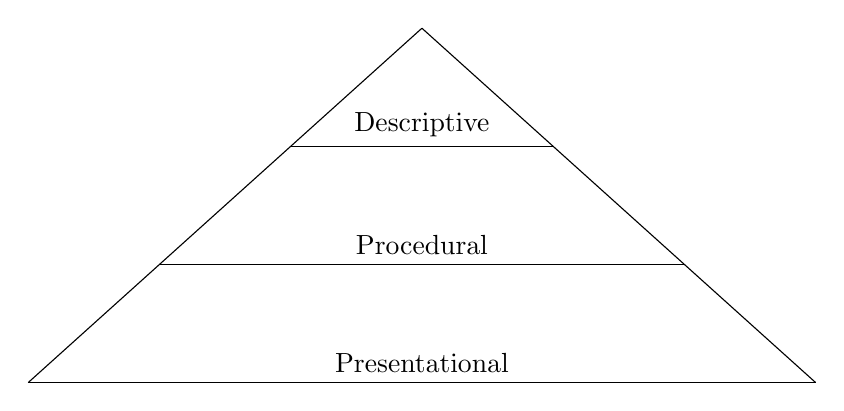
\begin{tikzpicture}
  \coordinate (Descriptive) at (-5,0) {};
  \coordinate (Procedural) at ( 5,0) {};
  \coordinate (Presentational) at ( 0,4.5) {};
  \draw (Descriptive) -- (Presentational);
  \draw (Procedural) -- (Presentational);
  \foreach \y/\Descriptive in {0/Presentational, 1/Procedural, 2/Descriptive} {
      \draw ($(Descriptive)!\y/3!(Presentational)$) -- ($(Procedural)!\y/3!(Presentational)$) node[midway,above] {\Descriptive};
  }
  \end{tikzpicture}

\caption{A hierarchy of markup language abstraction.}
\label{fig:markup-types-hierarchy}
\end{figure}


% TODO: We are talking about _instances_ of documents, which is why we are not regarding abstract markup languages.











\section{Nested markup}
\label{sec:nesting}
\paragraph{A fundamental feature of (many) descriptive markup languages is the ability to nest elements such that a larger set of semantics is expressible than with merely the isolated elements themselves.} In many markup languages, this is implemented as the ability to nest elements in hierarchies. It is, of course, possible to nest without the use of hierarchies, but as \citet*{durand} point out, hierarchical nesting the the strategy that has been most prominent. Perhaps because there exist many conflicting suggestions on how to approach non-hierarchical nesting. Some of these are outlined by \citet{durand} but an extensive amount of papers have been written on the matter of non-hierarchical nesting \footnote{http://xml.coverpages.org/hierarchies.html}. Still, today, hierarchical document structures enjoy the most widespread use. Consider, for example, the large family of XML-based languages such as HTML. The generic container element \texttt{<div>}, may, e.g., be nested arbitrarily deep inside any other \texttt{<div>} element.



To enforce the difference between nesting and not, consider the following, languageted, paragraph of text\footnote{This thesis ignores discussions of the treatment of whitespace.}, as depicted in Figure \ref{fig:mixed-content-paragraph}.


\begin{figure}[h]
\centering
\fbox{
The color \underline{is \textbf{now}} \sout{red}.
}
\caption{An example paragraph with languageting.}
\label{fig:mixed-content-paragraph}
\end{figure}


Naively analyzed, the paragraph consists of the four unique ``token types'' (1) plain-text, (2) underline, (3) bold-underline, and finally (4) strikethrough.





\begin{figure}[h]
  \centering
  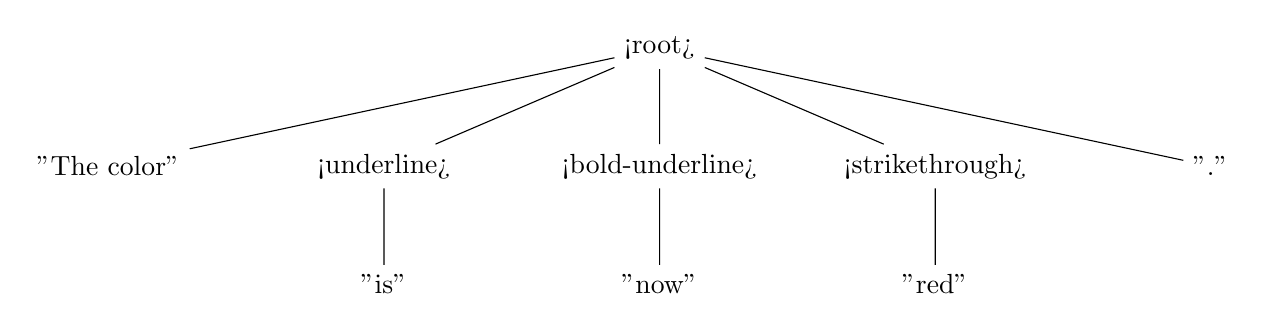
\begin{tikzpicture}[
    tlabel/.style={pos=1,right=2pt,font=\footnotesize\color{red!70!black}},
    sibling distance=3.5cm,
  ]
  \node {<root>}
  child {node {"The color"}}
  child {node {<underline>}
    child {node {"is"}}
  }
  child {node {<bold-underline>}
    child {node {"now"}}
  }
  child {
    node {<strikethrough>}{
      child {node {"red"}}
    }
  }
  child {node {"."}}
  ;
  \end{tikzpicture}

  \caption{Pre-order tree representation of Fig. \ref{fig:mixed-content-paragraph}.}
  \label{fig:mixed-content-flat-tree}
\end{figure}



Less naïvely analyzed, two of words are underlined, but one of the words that are underlined is actually both underlined and bold. This is an example of a situation where nesting may be employed to express a thing as a mere combination of two existing things, rather than as a completely new thing. Consider the difference between the non-nested tree representation in Figure \ref{fig:mixed-content-flat-tree} and the nested tree representation in Figure \ref{fig:mixed-content-tree}.


\begin{figure}[h]
  \centering
  \begin{tikzpicture}[
    tlabel/.style={pos=1,right=2pt,font=\footnotesize\color{red!70!black}},
    sibling distance=3cm,
  ]
  \node {<root>}
  child {node {"The color"}}
  child {node {<underline>}
    child {node {"is"}}
    child {node {<bold>}
      child {node {"now"}}
    }
  }
  child {
    node {<strikethrough>}{
      child {node {"red"}}
    }
  }
  child {node {"."}}
  ;
  \end{tikzpicture}

  \caption{Pre-order tree representation of Fig. \ref{fig:mixed-content-paragraph} employing nesting.}
  \label{fig:mixed-content-tree}
\end{figure}






\subsection{The importance of nesting}
\paragraph{Without the ability to combine tokens, the number of terminal tokens in a hypothetical lexer would exponentially increase for every introduced token.} Nesting, allow, an infinite language to be expressed through a finite set of tokens. Nesting must thus, be considered a fundamental, and necessary, property of any pragmatically useful markup language.

Below, three arguments will be given in order to enforce the importance of nesting.


\paragraph{(1) The potential difference in semantics between the nested, i.e. the implicit, and the non-nested, i.e. the explicit, is irrelevant.}
This argument stems from the assumption that preservation of semantic difference is more important than preservation of semantic equivalence (as outlined in the Section \ref{sec:difference-is-more-important-than-equivalence}).

Consider for example chapters and subchapters. One explicit way of distinguishing between the two would be to introduce one syntactic keword denoting a chapter, and another denoting a subchapter. This is an explicit approach. An implicit approach however would be to argue that any chapter ``inside'' of another chapter should be considered a subchapter. In this latter case, only the syntactic keywords for denoting a chapter are required.


\paragraph{(2) Nesting can reduce the number of required terminal tokens.}
Assume two unique terminal tokens -- $A$ and $B$. Then assume a language where a string can semantically belong to either class A, class B, or simultaneously to both class A and and class B. Without the power of nesting, this requires the introduction of a third explicit token that represent the the combination of these two - i.e. $AB$.

However, introducing a single token is not sufficient if the starting point is a set of three unique terminal tokens, rather than, as in the example, two. Subsequently, far from sufficient if the starting point is a set of 100 unique terminal tokens.


\begin{figure}[h]
\centering
\fbox{
Lexing \underline{without \textbf{\sout{parsing} may}} \sout{make} \textbf{life \sout{oh so} \underline{cumbersome}}.
}
\caption{A string exhausting the combinations of $\{bold, underline, strikethrough\}$.}
\label{fig:mixed-content-paragraph-complex}
\end{figure}


Extracting the tokens from Figure \ref{fig:mixed-content-paragraph}, one reaches the set described by Equation \ref{eq:tokens-as-subset} (assuming plain-text is ignored) and can then trivially construct a string, such as in Figure \ref{fig:mixed-content-paragraph-complex}, that exhaust all possible combinations.



\begin{equation}
\{B, U, S\} = \{bold, underline, strikethrough\}
\label{eq:tokens-as-subset}
\end{equation}



Mathematically, the total number of terminals in a grammar that allow combinations of unique terminal tokens, correspond to the number of $k$-combinations for all $k$, of $n$, where $n$ is the number of unique terminal tokens before combining. In other words: the total number of tokens is the number of possible subsets of the set of unique terminal tokens. Expressed in Equation \ref{eq:formula-all-subsets}.

\begin{equation}
\sum_{0\leq{k}\leq{n}} {n \choose k} = 2^n
\label{eq:formula-all-subsets}
\end{equation}

Since plain-text is considered the token that is present when all the other tokens are absent, this means plain-text must not be considered a token possible to combine. In other words plain-text will always be represented by a one, single, token, regardless of the number of other tokens within a set. Since the result of Equation \ref{eq:formula-all-subsets} also include the empty set, this fits naturally to the description of the plain-text token.

Applying the formula of Equation \ref{eq:formula-all-subsets} to Figure \ref{fig:mixed-content-paragraph} yields the subsets depicted in Formula \ref{eq:all-subsets-of-example}.

\begin{equation}
\{\{\};\{B\};\{U\};\{S\};\{BU\};\{BS\};\{US\};\{BUS\}\}
\label{eq:all-subsets-of-example}
\end{equation}


However, as many markup languages allow authors to permute the base tokens and not merely combine them, it is important to realize that Equation \ref{eq:all-subsets-of-example} only combines, and that the number may thus, in fact, need to be much higher. Consider for example the subtle distinction between an \textit{\textbf{italicized bold}} string and a \textit{\textbf{bolded italic}} string.

Whether such a distinction would matter in a language is of course dependent on that particular language, and might even vary on a per-token-basis within that particular language. While the distinction might be irrelevant in the example above (combining bold and italics), consider instead the semantic distinction between a \emph{paragraph in a figure} and a \emph{figure in a paragraph}.

Assuming a language where all tokens may be permuted and not simply combined, the required total number of tokens, would correspond to the number of $k$-permutations of $n$, for all $k$, where $n$ is the number of unique terminal tokens before combining (as depicted in Formula \ref{eq:formula-permutations}).


\begin{equation}
\sum_{0\leq{k}\leq{n}} P(n,k) = 
\sum_{0\leq{k}\leq{n}} \frac{n!}{(n-k)!}
\label{eq:formula-permutations}
\end{equation}

Applying the formula of Equation \ref{eq:formula-permutations} to the set of Figure \ref{eq:tokens-as-subset}, yield 16 tuples (as depicted in Equation \ref{eq:all-tuples-calculation}), where the resulting tuples depicted in Equation \ref{eq:all-tuples}.



\begin{equation}
\begin{split}
\frac{3!}{(3-3)!} + \frac{3!}{(3-2)!} + \frac{3!}{(3-1)!} + \frac{3!}{(3-0)!} = 
16
\label{eq:all-tuples-calculation}
\end{split}
\end{equation}



In summary, a language with three terminal tokens, where all permutations are allowed, must actually contain $16$ terminal tokens. In a language of four tokens, the number becomes $65$. Obviously this is absurd, a thus, a good reason as to why nesting is such an important corner stone of markup languages. Because it allow languages to omit the explicit use of terminals in favor of implicit hierarchies.

It is important to realize that all these calculations are based upon a nesting depth of 1. If semantics would differ and deeper levels then even more tokens would be required.




\begin{equation}
\begin{split}
\{
(); \\
(B);
(U);
(S); \\
(B,U);
(B,S);
(U,B);
(U,S);
(S,B);
(S,U); \\
(B,U,S);
(B,S,U);
(U,B,S);
(U,S,B);
(S,U,B);
(S,B,U)
\}
\label{eq:all-tuples}
\end{split}
\end{equation}


% TODO: Call these ``derived'' tokens????




\paragraph{(3) Nesting enable infinite languages over finite words.}
This can be easily understood by contemplating the language of infinitely nestable chapter tokens. In other words, a markup language in which every chapter nested inside of another chapter denotes a sub-chapter of the chapter level of the previous chapter. In other words the first time a chapter appears, it is a top-level chapter. When a chapter appears within that other chapter it is a sub-chapter. When a chapter appears within that sub-chapter, it denotes a sub-sub-chapter. And so forth, into infinity.

in terms of formal grammars, nesting allow non-terminals to, directly, or indirectly, produce themselves. Thus, enabling languages to be infinitely complex, even through finite sets of terminal tokens. This is, obviously, a common, and powerful, phenomenon in regards to markup languages. As without nesting, it would be impossible to achieve infinite languages over finite words.

Another example is the Dyck\footnote{http://en.wikipedia.org/wiki/Dyck\_language}-like languages of infinite, balanced parentheses, as shown in Figure \ref{fig:mixed-content-nesting}.

% TODO: I'm on some very thin ice over here.


\begin{figure}[h]
\centering
\fbox{
Consider (the (infinite (nesting) of (parentheses))).
}
\caption{A Dyck language with balanced parentheses.}
\label{fig:mixed-content-nesting}
\end{figure}







\subsection{Non-hierarchical nesting}
\label{sec:non-hierarchical-nesting}
It is important to understand that this thesis employ and endorse the hierarchical model of nesting for delimitational and pragmatic reasons. This thesis argue that the necessary property, is nesting, but not necessarily hierarchical such. Since there (as previously discussed) is disagreement in the community, and exist a number of conflicting papers\footnote{http://xml.coverpages.org/hierarchies.html}, with no consensus, on how to approach non-hierarchical nesting, this thesis is delimited to nesting of the hierarchical kind.











\section{Mixed content}
\label{sec:mixed-content}
\paragraph{Mixed content allow text to be interpolated with semantic descriptions, and can be used to distinguish languages suitable for document authoring, from languages merely intended for data modeling.} The former (i.e. document authoring) can be considered a specialization of the latter (i.e. data modeling). As this thesis is only concerned with understanding conversion between document authoring languages, and not between the much larger body of data modeling languages, it is important to find a way of distinguishing between the two.

\paragraph{The essential difference between documents, and data, is that documents are sequentially ordered whereas data is merely structured.} As documents may indeed exhibit non-sequential properties, one must consider whether the abstract idea of some particular data is intended to be consumed sequentially or not. Even if some abstract idea have multiple sequential interpretations, it should be allowed to be considered a document, and thus even very structured data may be considered documents. Such a high level of structure is for example utterly useful when intending to spawn multiple interpretations from an input document in order to output multiple different manifestations.

Since documents must, necessarily, house sequential properties, a language in which the document is expressed must, necessarily, allow for sequentiality.

\paragraph{Mixed content essentially encapsulate the idea that documents are sequential series of interpolations between the semantically specified and the semantically unspecified.} In other words, that the semantics of some free flowing text may, at any time, be extended with further semantic information. Consider for example the interpolation of the semantic information ``emphasize'' in the example paragraph below.

\begin{lstlisting}
<quote>I'm sorry, but I don't <bold>want</bold> to be an emperor.</quote>
\end{lstlisting}

In other words, mixed content is a way of allowing descriptive markup languages to maintain sequentiality, and not introduce procedurality, while still enabling semantic decorations at any point in a document.

% TODO: Use and refer to the terms used by H. Schöning (2001) -- Tamino a DBMS for XML.

\paragraph{The first official W3C working draft of XML already contained the idea of what was referred to as ``mixed content''.}(1996)\footnote{http:\/\/www.w3.org/TR/1998/REC-xml-19980210\#sec-mixed-content} Simplified, the idea was that an element may either contain a string of text, or another element, or any combination of the two. In (1998) W3C published a recommended specification of XML 1.0, where the concept of mixed content was expressed as a grammar in Extended Backus-Naur Form (subsequently referred to as EBNF) as follows\footnote{Part of the production for the non-terminal ``content'' has been omitted in favor of readability.}.

\begin{lstlisting}
element ::= EmptyElemTag | STag content ETag 
content ::= (element | CharData)*
\end{lstlisting}

To summarize the above grammar -- any non-terminal \texttt{element} can either produce an \texttt{EmptyElemTag} (i.e. self-closing tag), or the set of a \texttt{STag} (i.e. opening tag) followed by \texttt{content}, followed by an \texttt{ETag} (i.e. closing tag). The non-terminals \texttt{EmptyElemTag} (e.g. \texttt{<foo/>}), \texttt{STag} (e.g. \texttt{<foo>}) and \texttt{ETag} (e.g. \texttt{</foo>}) will terminate without any risk of indirect recursion back to the non-terminal \texttt{element}. The non-terminal \texttt{content} is the one interesting to this example.

The XML 1.0 (1998) specification use the following flavored syntax\footnote{This is of course merely a partial extraction of the syntax used in the specification.} of EBNF. The character ``pipe'' (|) represent an \texttt{XOR} choice such that \texttt{A | B} match ``A or B but not both''. The character ``star'' (*) is used as a ``Kleene Star'' such that \texttt{A*} matches ``zero or more occurrences of A''. Parentheses is used to group expressions such that the two mentioned operators can be used on an expression group.

Essentially, the non-terminal \texttt{content} can either produce a new \texttt{element} (causing potential indirect recursion) or \texttt{CharData} (i.e. a string), any number of times. Subsequently allowing for any combination of any length of the two.

In other words, the above EBNF specify that any XML element may contain any interpolation of XML elements and strings.

\paragraph{In terms of formal grammars -- mixed content enable the free text terminal token to be interpolated with tokens of semantic description.} Not with continuous precision, but down to the level of each character of a string. After all, text is not syntactically continuous, but rather discretely bound to its atoms -- the characters of a language. In other words, any number of semantic descriptions must be able to be applied to any character in a string, at any point in the string.



\subsection{Determining support for mixed content}
\paragraph{Mixed content cannot be, unanimously, expressed in languages that lack a canonical way of expressing it.} Remember that the definition followed in this thesis, is that languages that support mixed content, support sequential interpolation of semantic keywords in otherwise semantically unspecified text. This thesis propose two tests, one can run, in order to determine whether a language is suitable for mixed content or not.

\begin{enumerate}
\item All valid strings in the language, must also be valid mixed content\footnote{Some strings may of course not exhibit mixed content, but they must in either case be valid strings according to the parsing strategy of mixed content of that language.}. As depicted using Venn notation in Figure \ref{fig:mixed-content-venn}.
\item All sequentiality must be preserved.
\end{enumerate}


\begin{figure}[h]
\centering
\begin{subfigure}{.4\textwidth}
  \centering

  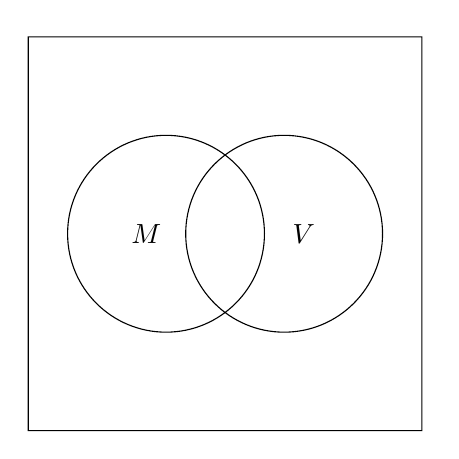
\begin{tikzpicture}[fill=gray]
    \draw (-.75,0) circle (1.25) (1,0)  node [text=black] {$V$}
          ( .75,0) circle (1.25) (-1,0)  node [text=black] {$M$}
          (-2.5,-2.5) rectangle (2.5,2.5) node [text=black] {};
  \end{tikzpicture}
  \caption{Not all valid JSON ($V$) is valid mixed content ($M$).}
  \label{fig:mixed-content-venn-json}
  
\end{subfigure}%
\begin{subfigure}{.4\textwidth}
  \centering

   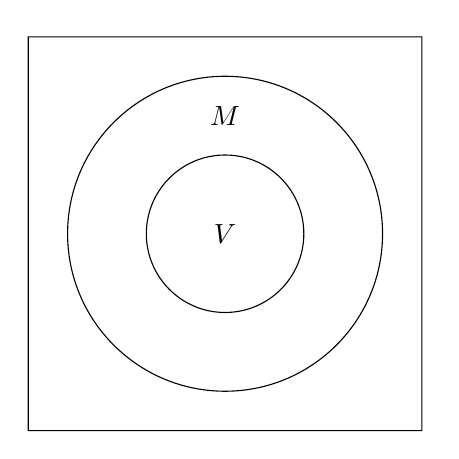
\begin{tikzpicture}[fill=gray]
    \draw (0,0) circle (2) (0,1.5)  node [text=black] {$M$}
          (0,0) circle (1) (0,0)     node [text=black] {$V$}
          (-2.5,-2.5) rectangle (2.5,2.5) node [text=black] {};
  \end{tikzpicture}
  \caption{All valid XML ($V$) is valid mixed content ($M$).}
  \label{fig:mixed-content-venn-json}
  
\end{subfigure}
\caption{The relationship between valid strings in a language and valid mixed content strings.}
\label{fig:mixed-content-venn}
\end{figure}



JSON is an example of a language unsuitable for mixed content, as it breaks the second rule, and thus serves as an example on why both rules are necessary. The problem essentially is that the object notation of JSON is a non-sequential key-value-store. If objects in JSON were sequential it would be possible, yet awkward, to express mixed content in JSON.

\begin{figure}[h]
\begin{lstlisting}
[
  "root",
  "The color ",
  [
    ["line", "is", { "key": "red" }]],  // Deliberate use of different syntax..
    ["line", "and", ["key", "blue"]]],  // ..to exemplify the different alternatives
  ],
  "now."
];
\end{lstlisting}
\caption{Attempting to express Figure \ref{fig:mixed-content-paragraph} in JSON.}
\label{fig:mixed-content-json}
\end{figure}

The attempt to express mixed content in JSON, in Figure \ref{fig:mixed-content-json}, actually produce an unambiguous mixed content if one employ the following rules. Let all arrays be parsed as non-binary s-expressions where the first element is always the semantic description of the element. Let then all objects be sequences, where all keys are the semantic descriptions of the element given as a value. These simple rules actually allow any valid string of JSON, to be parsed as mixed content. The problem however, again, lies in that we are violating the specification of JSON when saying that all objects must be sequential. Thus the second rule cannot be fulfilled, and thus JSON cannot be considered suitable for mixed content.

\begin{figure}[h]
\begin{lstlisting}
<root>
  The color
  <line>is <key>red</key></line>
  <line>and <key>blue</key></line>
  now.
</root>
\end{lstlisting}
\caption{The XML equivalence of the JSON string in \ref{fig:mixed-content-json}. Line-breaks are only inserted for the sake of readability.}
\label{fig:json-mixed-content-xml-equivalence}
\end{figure}

In fact, since JSON objects are non-sequential, no parsing strategy of JSON will ever produce valid mixed content according to the definitions above. Unless, of course, one significantly alter the semantics of the object notation and claim it to be something like a substring randomizer.



%\paragraph{Ambiguity in JSON mixed content}
%TODO: Show examples of how lexing and parsing JSON mixed content may create different parse trees. %Ambiguity.



\subsection{The importance of mixed content}
\paragraph{Almost three out of four documents on the ``XML web'' utilize mixed content.} This is what \citet{mignet} found in  study ``the subset of the Web made of XML documents only''. More accurately, the study found that 72\% of all documents utilize mixed content. \citet{mignet} conclude that they've invalidated the folklore of underestimating the importance of mixed content in XML.

Given the higher presentational orientation of HTML (the de facto language of the web), in relation to XML, it is reasonable to assume that the number of documents on the web that utilize mixed content could be much higher, than what was found by \citet{mignet}, if also considering HTML.

As a more informal argument, anyone who has ever authored a sequential document in a markup language of the XML-family (counting improper subsets such as HTML5) will house some appreciation of how absurd document creation would be without mixed content.





% TODO: Should I exemplify more? Do we need to show JSON problems using parse trees? Why else are we showing parse trees?
% \subsection{Old stuff TODO}
% Markup is not just data transportation. An explanation as to why object notation is a subset of annotations. Meaning that languages % like \texttt{JSON} are too data-centric and can consequently not, in any sensible manner, be used for manual document authoring. \% texttt{XML} for example can be used for data transport, but in this thesis we'll focus on its markup properties. Consequently also%  % ignore languages like \texttt{JSON}, \texttt{YAML} etc.% 
% 
% Maybe we can even use parse-tree's to symbolize the problem. To show that it is not possible to unambiguously represent mixed content. One needs to perform computation on the parse tree to derive the data.














\section{Generic Identifiers and Validity}
\label{sec:theory:generic-identifiers-and-validity}
\DeclareFixedFootnote{\refXMLspec}{http://www.w3.org/TR/WD-xml-961114}

\paragraph{The fact that authors of XML documents can name their elements almost arbitrarily is enabled by, what is commonly referred to as, Generic Identifiers (GI's), and give authors the power of languages over infinite words, but also shifts the responsibility of document validation, from the language designer, to the document author.}

Generic Identifiers was already present in GML, and as XML is a subset of SGML\refXMLspec, and SGML ascended from GML\footnote{http://www.sgmlsource.com/history/roots.htm}, it is only reasonable to assume that the concept has been inherited rather than reinvented.

According to \citet{goldfarb}, GML was designed upon two ``novel postulates''. Firstly that (1) markup should describe a document's structure rather than the processing to be performed. A document once expressed descriptively should suffice for all future processing. Secondly that (2) markup should be rigorous, such that programs can be used for processing documents.

% TODO: Here it becomes really obvious that already then one knew one should only need a single input document.

The ingenious move of GML , according to \citet{goldfarb}, was to only let the markup language cover the first point of the two above. In other words, that GML allowed an author to describe a document's structure in any way she see fit, using the mnemonic tag -- i.e. GI's. In order to achieve the second goal, \citet{goldfarb} explained that, GML documents ought to be coupled with GML Models. Where the GML Model notation essentially is a notation derived from the Backus Naur Form-notation (BNF), but where the intent is to define the set of all valid elements (rather than string tokens).

Perhaps, GML models can be seen as the forefather of the Document Type Definition (DTD) that were introduced into SGML and followed into the subset XML\footnote{http://www.w3.org/TR/WD-xml-961114\#dt-dtd}.

\begin{figure}[h]
\centering
\begin{lstlisting}
:p.This added information, called :q.markup::q., serves two purposes: 
:ol.
:li.it separates the logical elements of the document; and 
:li.it specifies the processing functions to be performed on those elements. 
::ol.
\end{lstlisting}
\caption{An example of GML syntax by \citet{goldfarb}.}
\end{figure}




\subsection{Tag-validity and type-validity}
%TODO: Remember to use this piece of information!!
\label{sec:tag-validity-type-validity}
\DeclareFixedFootnote{\refSGMLspec}{http://xml.coverpages.org/wg8-n1929-g.html}

\paragraph{In SGML an explicit distinction was made between, what was called, tag-validity and type-validity\refSGMLspec.} GML Models made no such distinction and both concepts were thus instead encompassed into the idea of GML Models.

The SGML specification\refSGMLspec defined a type-valid SGML document as a document conforming to it's encompassing DTD. Subsequently defined a tag-valid SGML document to be a document that is ``fully tagged''. A document were to be considered ``fully tagged'' if every element in the document is composed of a start-tag with a generic identifier and a corresponding end-tag.

In essence, tag-validity describes whether a particular document is a syntactically valid document within the language in question (e.g. XML or SGML). Whereas type-validity describes whether that particular document is semantically valid within the given domain (usually specified via a DTD). Both are of course important for, as \citet{goldfarb} puts it, rigor.


\subsection{The importance of Generic Identifiers}
\label{sec:importance-of-generic-identifiers}
\paragraph{According to \citet{goldfarb}, the classic markup language Scribe (constructed by \citet{reid}) manage to avoid procedural markup completely (i.e. stay descriptive), much because of the effective use of Generic Identifiers (GI's).}

If then, as already established in Section \ref{sec:abstraction-hierarchy}, it is desirable to reach a state where all manually authored markup is descriptive, then GI's seem like an invaluable tool.

\paragraph{Generic identifiers enable languages over infinite words.}
Consider, how the domain of descriptive markup languages can be divided into two sub-domains. One in which GI's exist, and element names may be made up on the fly, by the document author. Then another, in which GI's do not exist, that consequently is delimited by a fixed number of identifiers.

If both languages exhibit the nesting property, then both are infinite languages. However, one is an infinite language over finite words, and the other is an infinite language over infinite words. In other words, their relative expressiveness differ, and consist of different infinities.

This means, that the cardinality of the set of possible expressions in an infinite language over infinite words, must be greater than that of an infinite language over finite w ords.

\paragraph{With generic identifiers, authors have an infinite number of semantic differentiations. }
This means, that regardless of how complex some thing may be, an author can always reduce the complexity by simply denoting this thing through some generic identifier. Thus, all things can be semantically denoted at their highest possible level of abstraction.

Consider for example that one wants to apply some series of semantic rules to a number of given strings in order to convey the concept highlighting text. Assume, that these rules can be expressed as the combination of the three tags \texttt{<bg>}, \texttt{<emph>}, and \texttt{<bold>} (see Figure \ref{fig:gi-abstraction-before}). While it is of course entirely possible to state these three rules each and every time one wish to highlight a portion of the document, it would be significantly less error-prone to invent an abstraction, such as e.g. \texttt{<highlight>} and then simply use the abstraction at all places (see Figure \ref{fig:gi-abstraction-after}).

\begin{figure}[h]
\centering
\fbox{
\texttt{
  <bg=''yellow''></emph><bold>Some highlighted text.</bold></emph></bg>
  }
}
\caption{A fictive example, expressed in XML, of a set of elements an author may use repeatedly. Subsequently a good candidate for being replaced by a generic identifier.}
\label{fig:gi-abstraction-before}
\end{figure}

\begin{figure}[h]
\centering
\fbox{
\texttt{
  <highlight>Some highlighted text.</highlight>
  }
}
\caption{A fictive example of how the complexity of Figure \ref{fig:gi-abstraction-before} is reduced by increasing the level of abstraction, through replacing a series of elements with a single, generic identifier.}
\label{fig:gi-abstraction-after}
\end{figure}


As there exist no limit of the number of elements an author can create, one has an infinitely large domain of semantic names to use. In other words, there will always be a new word one can choose in order to semantically describe some new semantic concept, and one thus never run the risk of ``running out of distinctions''.

\paragraph{The infinite set of words enables authors to push decisions into the future.} \citet{coombs} point out the same benefit in relation to Referential markup, which has already been detailed in Section \ref{sec:referential-markup}. However, the idea is that abstractions give authors the luxury of ignoring the specifics, and leave them for figuring out later. For example instead of deciding how a character such as, e.g. ``--'' should be languageted, the author simply employ some referential markup such as \texttt{\&mdash;}, and then in a later stage, in document conversion, the decision is made on what to replace the referential markup with. Naturally, GI's can be used in the same way as referential markup, as they simply allow one to reduce the specifics, in favor of the abstract -- by replacing convoluted orchestrations with names.

Using GI's, authors can choose to to distinguish between strings that one suspect belong to different semantic domains. Given that one cannot ``run out of'' semantic distinctions, no immediate problem is faced with employing too many distinctions. On the contrary, employing the line of thinking from the background chapter of this thesis, more semantic distinctions essentially mean higher semantic resolution. 

\paragraph{Generic Identifiers allow authors to mark up their documents with names that cognitively make sense to the individual.} As emphasized by \citet{krijnen}, many authors choose to write documents in some simple language (such as e.g. Markdown), and then convert their documents more complex languages (such as e.g. \LaTeX{}), for simple reasons such as preferred syntax. In order to aid less technical document authors in their migration from more problematic word processors (such as most modern GUI-based word processors), the author of this thesis argue that preferred syntactic structure plays an important role.

\paragraph{In the XML specification}\footnote{http://www.w3.org/TR/REC-xml/\#sec-logical-struct} Generic Identifiers are defined using EBNF notation as follows\footnote{Some parts of the EBNF example snippet are omitted (such as element attributes), and some altered (such as the letter range) to favor readability.}:

\begin{lstlisting}
element  ::=  EmptyElemTag | STag content ETag
STag     ::=  "<" Name ">"
ETag     ::=  "</" Name ">"
NameChar ::=  NameStartChar | "-" | "." | [0-9] | [A-Za-z] | ...
Name     ::=  NameStartChar (NameChar)*
\end{lstlisting}

The EBNF snippet can informally be described as follows. An element can either produce an empty element tag, or the set of a start tag some content and then an ending tag. A start tag must produce a set of balanced chevrons (i.e. $<>$) in which between a name must be produced. A name can produce a non-whitespace-containing string where some characters are not allowed as the first character. And so forth for the closing of the element. A couple of valid examples are outlined below:

\begin{lstlisting}
<Name>Jane</Name>
<birthDate>2040</birthDate>
<divider/>
\end{lstlisting}


















% % % % % % % % % % % % % % % % % % % % % % 
%
%
%
%   Theory: Document processing
%
%
%
% % % % % % % % % % % % % % % % % % % % % %

\section{A three-step model of document processing}
\label{sec:three-step-model}
\paragraph{Descriptive markup is, as outlined by \citet{goldfarb}, less trivial to process than procedural markup.} In order to process a procedural document, one essentially need to parse the document and, while doing so, carry out each processing instruction accordingly. In the case of descriptive markup, however, there exist a disconnect between a particular marked up string and its corresponding processing function. In other words, procedural markup, essentially, is, processing instructions, whereas descriptive markup is semantic delimitation. Thus, descriptive markup separate document processing from the document itself.

To formalize this disconnect, \citet{goldfarb} suggest a three-step model for document processing. The term document processing here refer to the idea of taking some document containing Generic Identifier's (GI's) as input, applying some set of processing functions, to produce some other document as output. The three steps of \citet{goldfarb} are (1) recognition, (2) mapping, and (3) processing. These are explained in closer detail below.

\paragraph{Recognition} refer to the idea of recognizing that some piece of the document string should be considered an element that is marked up. While not explicitly expressed by \citet{goldfarb} it seems reasonable to informally consider this step to be the step of lexing (tokenization) and parsing, where its output would to be the parse tree.

\citet{goldfarb} gives the example of an element with the generic identifier ``footnote''. In this step, the processing program would know that a substring is to be considered a ``footnote'', and, is thus semantically differentiated from all things that are not ``footnotes''. At this particular step of the three-step model, only semantic delimitation is carried out. Meaning that one knows that all footnote elements are footnotes, but one has no idea of what the semantic meaning of being a footnote is.

\paragraph{Mapping} refers to the idea of pairing processing functions with document elements (or to follow the analogy of the last paragraph -- semantic delimitations). \citet{goldfarb} continue on the previously mentioned example of ``footnotes'', by saying that the element now would be paired up with a processing function, such as e.g. one that collects the content encapsulated in the footnote element, only to later print it at the bottom of that page.

\paragraph{Processing} simply refer to the task of actually executing processing functions upon their respectively mapped elements. In other words, when an element has been identified, and mapped to some particular processing function, then the processing function is carried out.



\subsection{The importance of the three-step model}
\paragraph{Considering the XML eco-system, it becomes apparent how the three-step model of \citet{goldfarb} is applicable to tools that are highly useful today.} The recognition step is essentially carried out in all XML parsers. Considering the specific case of using XSLT to transform (in terms of this thesis: convert) documents, XPath could be used for traversing the parsed XML tree in order to locate some particular element (or set of elements) one wish to map some processing function, expressed in XSLT, to. Finally, the step of processing would be carried out by some XSLT processor such as, e.g. SAXON\footnote{http://en.wikipedia.org/wiki/Saxon\_XSLT}.

Given the widespread use of the XML-family of tools it is apparent that the three-step model of \citet{goldfarb} is not only readily applied, but also applied with success.





\section{Derived text}
\label{sec:theory:derived-text}
\paragraph{Derived text, as described by \citet{reid} in the paper that introduced Scribe, essentially refer to the idea that many parts of a document actually can be consider to be more or less complex derivations of other parts of the document.} Consider for example a table of contents, a bibliography, or a glossary. By strategically marking up a document, many parts can thus be generated from other parts of the document.

\citet{reid} describes the Derived Text facility of the markup language Scribe by exemplifying that any part of the text can be ``saved'' during the processing of a manuscript only to then be processed at certain ``collection points''.

While Scribe is an example of a descriptive markup language that enable derived text, it could also be implemented in a procedural markup language, perhaps as easily as through the use of variables.

\paragraph{Derived text is not referential markup, but rather in-language document conversions. } This, since (as briefly mentioned in Section \ref{sec:referential-markup}) referential markup represents one-to-one string inclusions from external sources (such as the inclusion of a file into another file), whereas derived text represents the idea of performing some number of conversions over elements in a document (such as the generation of a table of contents). Derived text conversions are thus, rather, to be considered equal to in-language document conversions (as outlined in Section \ref{sec:conversions-in-or-out-of-languages}), in the sense that one or multiple derived text conversions can be referred to as an in-language document conversion.



\subsection{Derived text across language boundaries}
\paragraph{Reusing text derivation strategies (i.e. code) across different languages is not unreasonable, but is also not trivial.} Consider for example the concept of a table of contents. While the syntactic implementations details may vary from language to language, the general idea of a table of contents is essentially the same regardless of language. Namely, to traverse the list of headings, into some given depth, and then produce a (perhaps indented) list of these headings.

As highlighted by \citet{krijnen}, coupling a mechanism of derived text to a given language makes it very hard to share derivation strategies (i.e. code) between languages.  \citet{krijnen} extend the commonly used universal document converter Pandoc\footnotePandoc{}, with the explicit intent of getting back ``the flexibility e.g. offered by the packages in the \LaTeX{} eco-system''. As Pandoc\footnotePandoc{} has a ``fixed'' intermediate language, \citet{krijnen} constructs a set of Haskell libraries that enable document authors to, essentially, ``map'' newly introduced elements of some language to the intermediate language. Consequently, if the author then writes text derivation strategies for that particular target of the intermediate language it means that all potential input languages that employ some mapping to that particular target will be able to reuse the text derivation strategy.

\paragraph{The paper by \citet{krijnen} essentially prove that it is possible allow document authors to merely ``map'' identifiers in an input language, to some intermediate language, and then employ derived text conversions on that intermediate language.} In other words, that it is possible to, with the help of ``mapping'', reuse text derivation strategies across language boundaries.

























% % % % % % % % % % % % % % % % % % % % % % % % % % 
%
%
%
%   EMPIRICS
%
%
%
% % % % % % % % % % % % % % % % % % % % % % % % % % 


\chapter{Empirics -- The artifact}



% % % % % % % % % % % % % % % % % % % % % % 
%
%   REQUIREMENTS
%
% % % % % % % % % % % % % % % % % % % % % %


\section{Requirements}
\label{sec:empirical-requirements}
\paragraph{The following paragraphs outline the requirements that were used when developing the artifact.} The requirements are derived from the Theory and Background chapters.

\begin{itemize}
\item \emph{Descriptive syntax} must be the only syntax allowed in input and intermediate languages. This, because, as outlined in Section \ref{sec:taxonomy-descriptive}, both \citet{coombs} and \citet{bray} seem in agreement on that procedural markup should be avoided in favor of descriptive.
\end{itemize}


\paragraph{In order to respect semantic resolution, i.e. attempt to only convert from languages with higher resolution to languages with lower resolution,} the input language must contain more semantic distinctions than all other conceivable output languages.

The following three are thus properties that must be supported by the input and intermediate languages. Firstly because they increase the number of possible semantic delimitations in languages, and secondly because they, as shown by \citet{coombs}, and by the XML specification\refXMLspec, have been, and are employed in widely used languages. If these properties where not available in the input language, the conversion tool would then risk having to operate at a lower semantic resolution than the output languages. The three properties of markup languages that are needed in order to respect semantic resolution are as follows:

\begin{itemize}
\item \emph{Nesting}, as outlined in Section \ref{sec:nesting}, enables infinite languages over finite words.
\item \emph{Generic Identifiers}, as outlined in Section \ref{sec:theory:generic-identifiers-and-validity}, enables languages over infinite words.
\item \emph{Mixed content}, as outlined in Section \ref{sec:mixed-content}, is available in common languages, such as XML\refXMLspec, and readily used, as showed by \citet{mignet}.
\end{itemize}



\paragraph{In order to facilitate the sharing of packages (i.e. code), for common conversions, across language boundaries, } all processing functions must follow the three-step model as outlined by \citet{goldfarb}, and all mappings must be possible to configure by an author. Using the terminology of the background chapter the suggestion is then that:

\begin{itemize}
\item \emph{Interpretation conversions} must be allowed to be proceeded by \emph{translation conversions}, so that the translation can map the elements of the input document to the appropriate processing functions of the interpretation conversion.
\end{itemize}




%\color{red}
%\subsubsection{Using configurations to map processing functions (TODO -- remove?)}
%\label{sec:applying-three-step-model-to-quad-b}
%In order to truly adhere to the second and third high-level goals (composability, and extendability), one sensible, and obvious, approach would be to allow conversions to be configured. Consider XSLT as en example. Assume one were to construct a package system (such as the package system of \LaTeX) or (perhaps even) a public package channel\footnote{A ``package channel'' refer here to the idea of a unified publicly accessible package system, such as e.g. \texttt{apt-get}, \texttt{RubyGems} or \texttt{npm}}. Consider now that authors are free to choose element names freely in XML. This mean it would either be utterly difficult for a package creator to assume the right names for some set of elements when constructing the package, or it would spawn a situation where document authors would have to constantly adapt to the names used in packages. This of course violates the second high-level goal as it makes the package-eco-system significantly less composable.

%One sensible alternative would be to apply the three-step approach to document conversion, proposed by \citet{goldfarb}. Applying this three-step process allow different intents to be left to different parts of the eco-system. Step one and two (recognition and mapping) would be carried out by the individual that aim to \emph{use} the package. Where the second step would allow the user to map the names of her elements onto the names of the elements in the ``processing function'' (PF) (i.e. the package). The package creator would thus create, only the PF. It is important of course that the PF would have to be created in a way such that it allows arguments to be passed, and thus mapped onto the variable element names within the PF.  Step three would be carried out by the conversion program itself.

%For the sake of standardization it would of course, and again, proper composability, it would of course make sense to standardize the way that a PF exposes its arguments.

%Figure \ref{fig:quad-b-with-three-step-process} depict the Quadrant B model refined with the property of this three-step process.

%\begin{figure}[h]
%  \centering
%
%  \begin{tikzpicture}[node distance=2.5cm]
%    \node (input)  [io] {$I$};
%    \node (P)      [process, right of=input] {$P$};
%    \node (output) [io,      right of=P] {$O$};
%
%    \node (C)  [ds,      above of=P, xshift=-1cm, yshift=-1cm] {\(C\)};  % {Configuration};
%    \node (F)  [ds,      above of=P, xshift=1cm,  yshift=-1cm] {\(PF\)}; % {Functions};
%
%    \draw [arrow] (input)  -- (P);
%    \draw [arrow] (P) -- (output);
%    \draw [arrow] (C) -- (P);
%    \draw [arrow] (F) -- (P);
%  \end{tikzpicture}
%
%  \caption{Quadrant B model refined with properties of the three-step model for document processing, by \citet{goldfarb}.}
%  \label{fig:quad-b-with-three-step-process}
%\end{figure}













% % % % % % % % % % % % % % % % % % % % % % 
%
%   PROPOSAL
%
% % % % % % % % % % % % % % % % % % % % % %

\color{black}
\section{Proposal}

\paragraph{In order to facilitate the sharing of packages (i.e. code) for common conversion tasks, the proposed solution is built upon a UNIX-like notion of pipes.}  The core command line tools in UNIX all read from standard in (stdin), and print to standard out (stdout)\footnote{http://en.wikipedia.org/wiki/Pipeline\_(Unix)}. This standardization enables synergy and make the whole of the core UNIX programs much greater than the sum of its parts.

The prototype proposal follows this notion of pipes, where input to, and output from, all conversion packages are simplified subset of XML, call it \texttt{flXML}. This goes for all conversions except the initial input, and the final output. The initial input is be given in an ad-hoc language constructed by the author of the document, and the final output document may break the language boundary of \texttt{flXML}, in order to be able to output to arbitrary languages such as PDF, CSV, RTF, etc..


\paragraph{In order to adhere to the last point of the requirements outlined in Section (\ref{sec:empirical-requirements}), interpretation conversions and translation conversions will be separated, and translation conversions will always be allowed to precede interpretation conversions.} This enables authors employ the concept of ``mapping'' from the three-step model of \citet{goldfarb}, and essentially enable authors to ``rename'' elements before sending their documents through some interpretation conversion package, in order for the interpretation conversion package to identify the elements correctly.

Figure \ref{fig:model-of-conversion-prototype-artifact} visualize the suggestion of possible ways of converting, and its properties are further explained below:

\begin{itemize}

\item $In$ represents the input document, written by the author in some ad-hoc arbitrary syntax (where double asterisk for example might denote the concept of bold, see Figure \ref{ex:numbered-headings-input} for an example).

\item $Out$ is the final target document, which may be expressed in an arbitrary language if the last step in a particular run was a $Translation$, that brought the document into another language. Only $Translations$ can produce documents in other languages.

\item $Parse$ is the process in which the document expressed in the arbitrary ad-hoc language gets translated into \texttt{flXML}. This is possible since the ad-hoc language designed by the author must be defined and supplied in a very simple JSON syntax (call it Flexup Definitions -- \texttt{fupd}) -- see Figure \ref{ex:numbered-headings-fupd} for an example. Each ``key'' in the JSON object of the Flexup definition will become the name of all elements captured by that particular syntax definition.

\item $Translation$ represents translation conversions, in other words, simple in-language conversions that may or may not be destructive. Translations are, as described in the background chapter, always one-to-one conversions, i.e. no elements are introduced and no elements are removed in such a conversion.

\item $Interpretation$ represents the package-sharable conversions. Since \texttt{flXML} is a subset of XML, interpretation conversion packages are written using XSLT. If an author wishes to use an interpretation conversion package that utilize elements with different names than the author currently have in the document, then the author can simply pipe the document through a $Translation$ and rename all elements in need of renaming.

\end{itemize}

\begin{figure}[h]
  \centering

  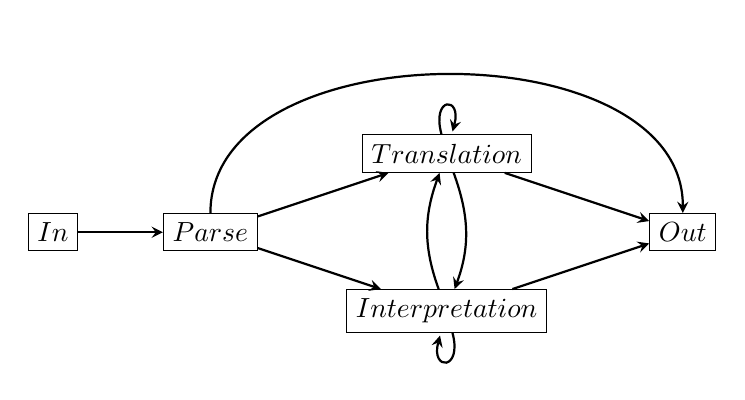
\begin{tikzpicture}[node distance=1cm]
    \node (i) [dot]                          {$In$};
    \node (P) [dot, right of=i, xshift=1cm]  {$Parse$};
    \node (o) [dot, right of=P, xshift=5cm]  {$Out$};
    \node (T) [dot, above of=o, xshift=-3cm] {$Translation$};
    \node (I) [dot, below of=o, xshift=-3cm] {$Interpretation$};

    \draw [arrow] (i) -- (P);
    \draw [arrow] (P) to[out=90, in=90]  (o);
    \draw [arrow] (P) -- (T);
    \draw [arrow] (P) -- (I);
    \draw [arrow] (T) -- (o);
    \draw [arrow] (I) -- (o);
    \draw [arrow] (I) to[out=110, in=-110] (T);
    \draw [arrow] (T) to[out=-70, in=70] (I);
    \draw [arrow] (I) edge[loop below]();
    \draw [arrow] (T) edge[loop above]();
  \end{tikzpicture}

  \caption{Model depicting possible conversion workflows of the proposed artifact.}
  \label{fig:model-of-conversion-prototype-artifact}
\end{figure}

A usage example of the program prototype is given in Section \ref{sec:usage-example}, and an example of the usage of pipes is depicted in Figure \ref{ex:numbered-headings-pipes-1}.














% % % % % % % % % % % % % % % % % % % % % % 
%
%   THE ARTIFACT
%
% % % % % % % % % % % % % % % % % % % % % %



\section{Usage example}
\label{sec:usage-example}

\paragraph{The developed prototype (call it Flexup) is, below, demonstrated through a usage example where a light-weight ad-hoc language is converted into HTML with auto-numbered headings and sub-headings.} The usage example is heavily inspired by \citet{krijnen}, who also add auto-numbering of headings, but use HTML as the input language.

\paragraph{The developed prototype is intended to illustrate the plausibility of the suggested approach, } and is thus, not intended to be considered production complete. Consequently, details such as alternative input syntaxes, or exhaustive regular expressions that actually lex all obscure characters correctly, are overlooked.


\paragraph{The scenario is such,} that an author has made up an arbitrary, small ad-hoc language and in this language written a document consisting of a number of headings and sub-headings. The aim is for the author to be able to convert this example file into an HTML file, that has running numbers prepended to all the headings.

Assume that the author types up a document, such as the one depicted in Figure \ref{ex:numbered-headings-input}. The document (referred to as a Flexup file, or a \texttt{fup}-file) is, as mentioned, expressed in an arbitrary ad-hoc language and in order for the Flexup prototype to be able to parse this language, the author also need to supply the grammar (referred to as a Flexup Definition, or a \texttt{fupd}-file). Flexup Definition files are expressed in JSON, and this particular Flexup Definition is depicted in Figure \ref{ex:numbered-headings-fupd}.

\begin{figure}[h]
\begin{lstlisting}
## First heading ##
And then some text

## A subheading ##
And some more text

## Last heading ##
And the last paragraph
\end{lstlisting}
\caption{Input document (\texttt{[document].fup})}
\label{ex:numbered-headings-input}
\end{figure}

Flexup Definition files essentially consist of a JSON object, where the keys are arbitrary names that describe some syntactical construct (i.e. an element). Each value corresponding to a key, is a very simple pattern that defines the syntactic structure of the element. Any number of characters, followed by a percentage sign, followed by any number of characters. The percentage sign is essentially a delimiter between the start tag and the end tag. Everything on the left of the percentage sign is considered the start tag, and everything on the right of the percentage sign is considered the end tag.

\begin{figure}[h]
\begin{lstlisting}
{
  "head"    : "##%##",
  "subhead" : "--%--"
}
\end{lstlisting}
\caption{Syntax definition (\texttt{[fupd].json})}
\label{ex:numbered-headings-fupd}
\end{figure}

Flexup Definitions will during the $Parse$ step of the conversion process (see Figure \ref{fig:model-of-conversion-prototype-artifact}) be converted into a Parsing Expression Grammar (PEG), that in turn will be generated into actual parsing code (that will be used to parse the Flexup file, expressed in the arbitrary syntax) using the JavaScript library PEG.js\footnote{https://github.com/dmajda/pegjs}. The PEG generated for this particular Flexup Definition is depicted in Figure \ref{ex:peg-grammar}.


\begin{figure}[h]
\centering
\begin{lstlisting}
start   = (element / text)*
content = (element / text)*
text    = t:[a-zA-Z \n]+          {return t.join("");}

/* * * EVERYTHING BELOW IS GENERATED * * */

element = STag1 c:content ETag1   {return {"head"    : c};}
        / STag2 c:content ETag2   {return {"subhead" : c};}

STag1   = "##"
ETag1   = "##"
STag2   = "--"
ETag2   = "--"
\end{lstlisting}
\caption{Example of Parsing expression grammar (in PEG.js syntax) generated from the Flexup Definition in Figure \ref{ex:numbered-headings-fupd}.}
\label{ex:peg-grammar}
\end{figure}

When the PEG, depicted in Figure \ref{ex:peg-grammar}, is, via the PEG.js library, converted into actual parse code, and then applied to the Flexup document (i.e. the input document) depicted in Figure \ref{ex:numbered-headings-input}, a parse tree is created in memory. The parse tree is nothing spectacular, but the one generated for this particular case is depicted in Figure \ref{ex:generated-parse-tree}.

\begin{figure}[h]
\begin{lstlisting}
[
   {
      "head": [" First heading "]
   },
   "And then some text",
   {
      "head": [" A subheading "]
   },
   "And some more text",
   {
      "head": [" Last heading "]
   },
   "And the last paragraph"
]
\end{lstlisting}
\caption{Parse tree generated from applying the PEG depicted in Fig. \ref{ex:peg-grammar}, to the Flexup file depicted in \ref{ex:numbered-headings-input}, by using PEG.js library.}
\label{ex:generated-parse-tree}
\end{figure}

What is more interesting, is how the prototype artifact then traverse this parse tree in order to construct the abstract syntax tree (AST). This AST is generated in form of the previously mentioned subset of XML referred to as flXML, and the one for this particular case is depicted in Figure \ref{ex:numbered-headings-flXML-ast-raw}.


\begin{figure}[h]
\begin{lstlisting}
<head>First heading</head>
And then some text

<subhead>A subheading</subhead>
And some more text

<head>Last heading</head>
And the last paragraph
\end{lstlisting}
\caption{First output file (\texttt{[ast].xml}), of the conversion process specified by the orchestration file in Figure \ref{ex:numbered-headings-pipes-1}}
\label{ex:numbered-headings-flXML-ast-raw}
\end{figure}

At the point of the AST, the author has the following three choices of action (as depicted in Figure \ref{fig:model-of-conversion-prototype-artifact}). The author can choose to (1) consider the AST the final output document and produce a physical file, or (2) run the file through a translation conversion, or (3) run the file through a interpretation conversion.

Assume that some other author has written a interpretation conversion package (i.e. some code), that searches a document for headings and subheadings and prepend numbers accordingly. Since interpretation packages in the suggested prototype must be written in XSLT, the package could look like the one depicted in Figure \ref{ex:numbered-headings-xslt-package}.

A discrepancy between the interpretation conversion code (Figure \ref{ex:numbered-headings-xslt-package}) and the current AST (Figure \ref{ex:numbered-headings-flXML-ast-raw}) will cause this particular package to not successfully traverse and number the AST. The problem is that the Flexup Definition caused the headings to be named \texttt{head} and the subheadings to be named \texttt{subhead}, whereas the interpretation conversion package expects them to be named \texttt{heading} and \texttt{subheading}. Thus, this is why translation conversion always are allowed to run before interpretation conversions. Translation conversions (call them Flexup Translations, or \texttt{fupt}) are given as JSON objects where each key denote the XPath of elements to search for, and a name to convert the name of all the matches to. An appropriate Flexup Translation for this particular case is outlined in Figure \ref{ex:numbered-headings-translation-fupt}.


\begin{figure}[h]
\begin{lstlisting}
<?xml version="1.0" encoding="utf-8"?>
<xsl:stylesheet version="1.0" xmlns:xsl="http://www.w3.org/1999/XSL/Transform">
  <xsl:template match="//heading">
    <heading>
      <xsl:value-of select="count(preceding-sibling::heading)+1"/>)
      <xsl:value-of select="." />
    </heading>
  </xsl:template>
  <xsl:template match="//subheading">
    <subheading>
      <xsl:value-of select="count(preceding-sibling::heading)"/> . 
      <xsl:value-of select="count(preceding-sibling::subheading)+1"/>
      <xsl:value-of select="." />
    </subheading>
  </xsl:template>
</xsl:stylesheet>
\end{lstlisting}
\caption{An XSLT package that traverses all headings and subheadings and prepends numbers accordingly.}
\label{ex:numbered-headings-xslt-package}
\end{figure}



\begin{figure}[h]
\begin{lstlisting}
{
  "//head"    : "heading",
  "//subhead" : "subheading"
}
\end{lstlisting}
\caption{Translation file.}
\label{ex:numbered-headings-translation-fupt}
\end{figure}


Having applied the Flexup Translation (Figure \ref{ex:numbered-headings-translation-fupt}) to the AST (Figure \ref{ex:numbered-headings-flXML-ast-raw}), it is then possible to run the XSLT interpretation conversion package (Figure \ref{ex:numbered-headings-xslt-package}). The result of applying the package is a new AST, now with numbered headers, depicted in Figure \ref{ex:numbered-headings-flXML-ast-numbered}.

\begin{figure}[h]
\begin{lstlisting}
<heading>1 First heading </heading>
And then some text

<subheading>1.2 A subheading </subheading>
And some more text

<heading>2 Last heading </heading>
And the last paragraph
\end{lstlisting}
\caption{Second output file (\texttt{[numbered].xml}), of the conversion process specified by the orchestration file in Figure \ref{ex:numbered-headings-pipes-1}.}
\label{ex:numbered-headings-flXML-ast-numbered}
\end{figure}


Again, the author can make the choice of applying further interpretation conversions, translation conversions, or simply writing the AST as a file to disk. In this particular usage example the goal was to end up with an HTML file, so consequently, another XSLT interpretation conversion package must be found, and all non-HTML elements must be translated into HTML-elements.

Figure \ref{ex:numbered-headings-translation-fupt-html-elements} illustrates a Flexup Translation that maps all elements that are not conforming to HTML, present in the AST of Figure \ref{ex:numbered-headings-flXML-ast-numbered}, to elements conforming to HTML. Applying this Translation to the current AST (Figure \ref{ex:numbered-headings-flXML-ast-numbered}) yields a new AST which only contains elements conforming to HTML.

Figure \ref{ex:numbered-headings-xslt-package-html-wrapper} illustrates a Flexup Interpretation that blindly wraps the entire AST in an HTML document. Applying this conversion to the new AST (Figure \ref{ex:numbered-headings-flXML-ast-numbered-html-fragment}) yields an actual HTML document, as depicted in Figure \ref{ex:numbered-headings-html-output}. The destination is now reached, and the document can be written to file. A complete conversion has been carried out.


\begin{figure}[h]
\begin{lstlisting}
{
  "//heading"    : "h1",
  "//subheading" : "h2",
  "//text()"     : "p"
}
\end{lstlisting}
\caption{Translation file.}
\label{ex:numbered-headings-translation-fupt-html-elements}
\end{figure}



\begin{figure}[h]
\begin{lstlisting}
<h1>1 First heading </h1>
<p>And then some text</p>

<h2>1.2 A subheading </h2>
<p>And some more text</p>

<h1>2 Last heading </h1>
<p>And the last paragraph</p>
\end{lstlisting}
\caption{Final output file (\texttt{[numbered].html}), of the conversion process specified by the orchestration file in Figure \ref{ex:numbered-headings-pipes-1}.}
\label{ex:numbered-headings-flXML-ast-numbered-html-fragment}
\end{figure}


\begin{figure}[h]
\begin{lstlisting}
<?xml version="1.0" encoding="utf-8"?>
<xsl:stylesheet version="1.0" xmlns:xsl="http://www.w3.org/1999/XSL/Transform">
  <xsl:template match="/">
    <!DOCTYPE html>
    <html>
      <head>
        <title>Example</title>
        <meta charset="utf-8">
      </head>
      <body>
        <xsl:value-of select="."/> 
      </body>
    </html>
  </xsl:template>
</xsl:stylesheet>
\end{lstlisting}
\caption{An XSLT package that wraps the whole document in an HTML document.}
\label{ex:numbered-headings-xslt-package-html-wrapper}
\end{figure}



\begin{figure}[h]
\begin{lstlisting}
<!DOCTYPE html>
<html>
  <head>
    <title>Example</title>
    <meta charset="utf-8">
  </head>
  <body>
    <h1>1 First heading </h1>
    <p>And then some text</p>

    <h2>1.2 A subheading </h2>
    <p>And some more text</p>

    <h1>2 Last heading </h1>
    <p>And the last paragraph</p>
  </body>
</html>
\end{lstlisting}
\caption{Final HTML output with numbered headings.}
\label{ex:numbered-headings-html-output}
\end{figure}



\begin{figure}[h]
\begin{lstlisting}
flexup.in("./[document].fup")                 // read input file
  .pipe(grammar("./[fupd].json"))             // parse using fupd
  .out("./[ast].xml")                         // write raw ast to disk
  .pipe(translation({                         // translation
    "//head"    : "heading",
    "//subhead" : "subheading"
  }))                    
  .pipe(interpretation("number-headings"))    // interpretation package
  .out("./[numbered].xml");                   // write ast to disk
  .pipe(translation({                         // translation
    "heading"    : "h1",
    "subheading" : "h2",
    "."          : "p"
  }))
  .pipe(interpretation("html-wrap"));         // interpretation package
  .out("./[numbered].html");                  // write output to disk
\end{lstlisting}
\caption{Orchestration file.}
\label{ex:numbered-headings-pipes-1}
\end{figure}


\paragraph{In order to orchestrate all of the steps above, the artifact has an API in which the pipes can be utilized.} The syntax of the orchestration file is heavily inspired by the ``streaming build system'' gulp.js\footnote{https://github.com/gulpjs}. All of the steps of the usage example in this section could be carried out through usage of the API, as depicted in Figure \ref{ex:numbered-headings-pipes-1}.

























% % % % % % % % % % % % % 
%
%
%
%   CONCLUSION
%
%
%
% % % % % % % % % % % % % 

\chapter{Conclusion}

\paragraph{Regarding Deliverable I -- a workflow that enable the respecting of markup resolution, sharing of packages, and the ability to produce any output language. } A workflow has been identified, and a prototype built.

\begin{itemize}
\item Regarding the enabling of respect for markup resolution, the conversion workflow utilize an input language that can be described as an ``infinite language over infinite words'', which in theory can describe any imaginable string. In the particular prototype implementation, the Flexup Definition facility is currently not competent enough to enable the author to express all domains of infinite words. It is sufficiently competent for expressing infinite words, but it is simply not competent for expressing \emph{all} the domains of infinite words. Importantly though, the domains of infinite words expressible by Flexup Definitions is still greater than the domains of infinite words expressible by languages such as XML. As, XML for example is bound to the syntactic construct of chevrons, whereas Flexup Definitions, are only coupled to the concept of a starting tag and an ending tag, without saying anything about what a starting tag and an ending tag should look like.

In other words, given that one starts from such an incredibly abstract language, and then can apply arbitrarily small conversions, it is only reasonable to assume that authors, through the use of Flexup, can respect markup resolution.

\item Regarding the sharing of packages, the differentiation between Interpretation conversions, and Translation conversions, seemingly makes a great difference in regards to ease of use, when sharing packages.

\item The ability to produce any conceivable output format is undoubtedly fulfilled, because of the delegation to the language XSLT. Given that XSLT is a Turing Complete language, it is thus safe to say that any string produced by a Turing Machine (or less) also can be produced by Flexup.
\end{itemize}


\paragraph{Regarding Deliverable II -- the identification of fundamental characteristics of a markup language in order to achieve a relative, high level of abstraction. }
\begin{itemize}
\item The fundamental characteristics identified are descriptive syntax (Section \ref{sec:taxonomy-descriptive}), nesting (Section \ref{sec:nesting}), mixed content (Section \ref{sec:mixed-content}), generic identifiers (Section \ref{sec:theory:generic-identifiers-and-validity}), and derived text (Section \ref{sec:theory:derived-text}) which together enable infinite languages over infinite words. It is obvious that there is no reason to assume that this list is neither the only way to reach such a language, nor the best. If one is to however, argue that a higher number of semantic delimitations is required than those in the identified set of infinite languages over infinite words, the author argue that further research in Formal Grammars must be identified, or carried out. As it currently stands, the identified properties are deemed more than sufficient, if seeking an input markup language with a relative, high abstraction.
\end{itemize}



\paragraph{In conclusion, there is good reason to believe that the concept of Markup Resolution plays an important role in the collectivizing of a markup conversion eco-system where the ultimate goal would be to achieve such a high level of package sharing that all users can achieve the notion of ``write once, publish everywhere''}.











% % % % % % % % % % % % % 
%
%
%
%   discussion
%
%
%
% % % % % % % % % % % % % 


\chapter{Discussion, Critique and Further Research}
Further use cases, and real world tests must be carried out before it is safe to say that the proposed approach of this thesis also is viable in practice, and not merely in theory.

It is also important to realize that many smaller implementation details have been put aside (as previously discussed in Section \ref{sec:usage-example}) during the development of this prototype. While there is currently no reason to suspect that anything significantly hazardous may hide in the implementation details, it would still be relevant to find out whether what seems theoretically reasonable in this thesis, also holds in practice, even when faced with all the implementation details.

Any new efforts to approach non-hierarchical markup would be highly valuable, as the eco-system in this thesis, as most other markup languages today, is not canonically able to deal with nested structures.

While the artifact implemented in this thesis indeed must be considered a prototype, the validating effect it has on the concept of Markup Resolution, must be taken seriously, and into further consideration. Many interesting questions still hide on the boundaries of linguistics, semantics, formal grammars, and philosophy.\\ \\

The prototype discussed in this thesis is distributed online as open source, package contributions are most welcome\footnote{https://github.com/chrokh/flexup}.













% % % % % % % % % % % % % 
%
%
%
%   BIBLIOGRAPHY
%
%
%
% % % % % % % % % % % % % 


\bibliography{bibliography}







\end{document}
